%\documentclass[lettersize,journal]{IEEEtran}
\documentclass[12p,AMS,STIX1COL]{WileyNJD-v5}
%\usepackage{amsmath,amsfonts}
%\usepackage{algorithmic}
%\usepackage{algorithm}
%\usepackage{array}
%\usepackage[caption=false,font=normalsize,labelfont=sf,textfont=sf]{subfig}
%\usepackage{textcomp}
%\usepackage{stfloats}
%\usepackage{url}
%\usepackage{verbatim}
%\usepackage{graphicx}
%\usepackage{cite}
\usepackage{enumitem}

%\hyphenation{op-tical net-works semi-conduc-tor IEEE-Xplore}
% updated with editorial comments 8/9/2021

%\usepackage{url}
%\usepackage{hyperref}
%\usepackage{subcaption}

%\usepackage{xspace}
\usepackage{xcolor}
%\usepackage{graphicx}
%\usepackage[noend]{algorithmic}
%\usepackage{algorithm}
%\usepackage[noend]{distribalgo}
%\usepackage{subfig}
%\usepackage{multirow}

\newcommand{\new}{\color{black}}
\newcommand{\old}{\color{black}}

\newcommand{\dc}[1]{\textit{\textcolor{red}{[rjs]: #1}}}
\newcommand{\fp}[1]{\textit{\textcolor{blue}{[fp]: #1}}}
\newcommand{\zm}[1]{\textit{\textcolor{red}{[ef]: #1}}}
\newcommand{\nm}[1]{\textit{\textcolor{red}{[nm]: #1}}}
\newcommand{\fd}[1]{\textit{\textcolor{magenta}{[fd]: #1}}}
\newcommand{\rg}[1]{{\color{red}RFG: #1}}

\newcommand{\ra}{\rightarrow}
\newcommand{\la}{\leftarrow}

\articletype{Article Type}
\received{00}
\revised{00}
\accepted{00}

\begin{document}

\title{Boosting Blockchain Consensus with Semantic Gossip}
%\title{Semantic Gossip for Efficient Blockchain Consensus}
%\title{Semantic Gossip to Scale Blockchain Systems}

\author[1]{Daniel Cason}
\author[2]{Ricardo Guimaraes}
\author[1]{Nenad Milosevic}
\author[1]{Patrick Eugster}
\author[3]{Zarko Milosevic}
\author[2]{Fernando Dotti}
\author[1]{Fernando Pedone}

\authormark{Author Name}
\titlemark{Author Guidelines}

\address[1]{\orgname{Universit\`{a} della Svizzera italiana},
\orgaddress{\state{Lugano}, \country{Switzerland}}}

\address[2]{\orgdiv{School of Technology}, \orgname{Pontif\'{i}cia Universidade Cat\'{o}lica do Rio Grande do Sul},
\orgaddress{\state{Porto Alegre}, \country{Brazil}}}

\address[3]{\orgname{Informal Systems},
\orgaddress{\state{Toronto}, \country{Canada}}}

 
\corres{<Corresponding author information>}

\presentaddress{<author present address information>} 

\abstract[Abstract]{%\fd{Title is provisory}
%
%\fd{Color legend: {\new text blue is new}. }
%
%\fd{{\old black is non modified from 'Paxos Gossip - maybe unuseful but here to check it and remember discussions.}}
%
%\fd{\color{violet} violet is existing text reviewed/modified to this paper}
%
%\fd{{\color{teal}parts in in green/teal is old text that is valid for this paper}.  
%   we have to see how to reuse or not.   this is to be considered a new paper, not an extension ... correct ?}
%
%\fd{Draft abstract to check if these are the main aspects.}
%\new
State Machine Replication has been extensively used to provide highly-available, strongly-consistent systems.  Modern systems often require additionally to scale to several nodes.  This is the case of 
%This is the case of several existing state machine replication based systems that have to span service provisioning to a wider geographical scope. 
several blockchains, that have to run consensus among dozens to hundreds of nodes.

Gossip allows to scale communication to larger sets of nodes and has been recently considered as communication layer to support consensus.
%
By their nature, both consensus protocols and gossip handle message losses and process failures.   This double redundancy means that it is not yet clear how efficient is to use gossip as a black building-box for consensus.

In this paper, we investigate these aspects in the context of blockchains.
%Due to their stringent scalability needs, this paper investigates    
%
The paper discusses how far redundancy can be eliminated without compromising consensus' safety and liveness.
%
Then it proposes to selectively eliminate redundancy considering the combined use of protocols.
%
To accomplish that, a cross layer mechanism is proposed that, while keeping modularity, uses message semantics from consensus at the gossip level to reduce overhead while forwarding messages.   With a prototype implementing the ideas, experiments with 32 and 128 nodes show that the mechanisms proposed respectively enhance throughput 1.24 $\times$ and  $3.42 \times$ while slightly reducing latency.  
% this is derived from pictures 3 to 6

Furthermore, we argue and show results that the proposed redundancy elimination mechanisms do not harm resiliency...

%\old


% Gossip-based consensus protocols have been recently proposed to confront the challenges faced by state machine replication in large geographically distributed systems.

% It is unclear, however, to which extent consensus and gossip communication fit together.

% On the one hand, gossip communication has been shown to scale to large settings and efficiently handle participant failures and message losses. 

% On the other hand, gossip may slow down consensus. 

% Moreover, gossip's inherent redundancy may be unnecessary since consensus naturally accounts for participant failures and message losses. 

% This paper investigates the suitability of gossip as a communication building block for consensus.

% We answer three questions: How much overhead does classic gossip introduce in consensus? Can we design consensus-friendly gossip protocols? Would more efficient gossip protocols still maintain the same reliability properties of classic gossip?
}

\keywords{Consensus, Gossip, BFT, Blockchains}

\footnotetext{title footnote...}

\maketitle


%%!TEX root =  report.tex
\section*{Draft Structure}
\fd{approximate size of proposed sections}
\small
\begin{verbatim}
Semantic Gossip and Tendermint

1. introduction                1,5 PAGES 
     similar elements
     
 2. background                 1,5 PAGES
        CHANGE SYSTEM MODEL
        CHANGE PROTOCOL TO TENDERMINT
  
 3. semantic gossip            2,5  PAGES     
     similar discussion
     
4. experimental evaluation     4  PAGES
     a-  topology analysis
     
     b- overall performance

     c- latency cdf 

     e- impact of signnatures
    
     f - resilience
                       
  5. related work              1     PAGES
  
  6. conclusions,              1,5   PAGES  
     references, bios  


  \end{verbatim}         
  \normalsize
               

%!TEX root =  report.tex
\section{Introduction}
\label{sec:intro}

Consensus is a fundamental abstraction in many fault-tolerant distributed systems~\cite{Lam78,schneider90}. 
Although consensus and state machine replication have been extensively studied under various conditions (e.g., synchrony assumptions, failure models), most studies consider consensus deployments with few participants. 
This is often justified because deployments with more than three or five participants are considered unrealistic.
Modern applications, however, challenge this belief by running consensus among many participants.
For example, some blockchain systems run consensus among dozens to hundreds of nodes~\cite{bucham18,buterin17,libra18}.

To accommodate a large number of participants, failures, and geo-distribution, some blockchain consensus protocols rely on gossip communication to handle the interactions of consensus participants \cite{Hyperledger,bucham18,buterin17,libra18}.
Gossip provides scalability and reliability guarantees by carefully designed rounds of message exchanges, in which processes communicate with subsets of other processes~\cite{demers87, Birman99}.
However, consensus protocols must also handle message losses and process failures due to their fault-tolerant nature.
This redundancy suggests that combining consensus and gossip protocols may lead to overhead.
In short, it is unclear how efficient it is to use gossip as a black building-box for consensus.  Our first research question is thus:

\vspace{-2mm}
\begin{itemize}
\item[] \emph{Can we identify and eliminate double redundancy situations of gossip and blockchain consensus combined, 
            without sacrificing consensus properties ?}
\end{itemize}
\vspace{-2mm}

To tackle this problem, we look into consensus and gossip combined.
The idea is to reduce the overhead of gossip by exploiting consensus semantics.  We identify concrete cases of unneeded redundancy and argue that its elimination neither harms safety nor liveness.  Thus, we propose ways to reduce redundancy selectively.
The proposed semantic gossip design optimizes gossip with two techniques, \emph{semantic filtering} and \emph{semantic aggregation}.
Semantic filtering allows the gossip layer to discard messages that have become redundant or obsolete according to the consensus logic.
Semantic aggregation shows that it is possible to aggregate several consensus messages into a single message without losing information. 
%
Although we use the Tendermint consensus protocol \cite{buchman2019latestgossipbftconsensus} to discuss ideas and design, the results generalize to Byzantine fault tolerant consensus protocols since the main aspects that enable filtering and aggregation are present in all of them. 
%
Having argued for the possibility and soundness of semantic filtering and semantic aggregation, the natural second research question addressed in the paper is:
\vspace{-2mm}
\begin{itemize}
\item[]  \emph{What are the performance benefits of augmenting a gossip-based communication substrate with semantic extensions?}
\end{itemize}
\vspace{-2mm}

This question is answered experimentally by comparing classical gossip and combinations of filtering and aggregation for a series of workloads and topologies. The proposed design keeps modularity while dealing with cross-layer aspects.
%
In a 128-node network, our experiments show that filtering and aggregation lead to a reduction of 80\% in the number of gossip messages exchanged per consensus instance, leading to improved throughput and reduced latency.

%When a single technique is adopted, there is a 40\% to 45\% reduction in the
%number of messages exchanged by processes via gossip, when compared with the
%classic, non-optimized, gossip communication substrate.

The performance advantage of semantic filtering and semantic aggregation is desirable as long as it does not come at the expense of the reliability that classic gossip provides.
We consider this aspect in our third research question: 

\vspace{-2mm}
\begin{itemize}
\item[]  \emph{Do the proposed semantic extensions compromise consensus resilience ?}
\end{itemize}
\vspace{-2mm}

To answer this question, we propose two experiments: 
in the first one we consider that a dishonest node remains silent and does not propose a block in its turn; 
in the second experiment we consider that a dishonest node omits part of the messages sent.   
In the first case, we gradually increase the number of dishonest nodes; in the second case we gradually
increase message drop.  In both cases the effect on baseline and proposed techniques are measured.
%
We found that Semantic Gossip-based Tendermint retains the resilience of gossip, ... \fd{ ... complete}


The remaining of the paper is organized as follows:
    Section~\ref{sec:background} defines the system model and introduces background information on gossip and Tendermint;
    Section~\ref{sec:semantic} proposes the design and implementation of Semantic Gossip in the context of blockchains, focussing the Tendermint protocol.  
    The semantic gossip mechanisms for filtering and aggregation are proposed,
    discussed to preserve consensus properties, and their design/implementation presented;
 Section~\ref{experiments} describes the evaluation of Tendermint using gossip, and Semantic Gossip communication.   The evaluation starts with a topologycal study to generalize observations, being follwed by throughput and latency assessment using different combinations of semantic gossip mechanisms.
    The last part brings an assessement of the resilience of Tendermint without and with Semantic Gossip, varying its mechanisms, in the presence of increasing number of byzantine nodes;
    Section~\ref{sec:relwork} surveys related work and Section~\ref{sec:conclusions} concludes the paper.
    

%!TEX root =  report.tex

\section{Background}
\label{sec:background}

This section introducess the system model and assumptions, provides the needed background 
on gossip communication, and presents the Tendermint blockchain consensus protocol.

\subsection{System model and assumptions}
\label{sec:model}

We consider a distributed system with an unbounded set of client processes $\mathcal{C} = \{ c_1, c_2, ... \}$ and a bounded set of server processes $\mathcal{N} = \{ n_1, ..., n_n \}$ we call nodes.
Processes communicate by exchanging messages and do not have access to a shared memory or a global clock. 
Processes can be \emph{correct} or \emph{faulty}. 
A correct or honest process follows its specification whilst a faulty process can present arbitrary (i.e., Byzantine) behavior. 

The system is partially synchronous: it is initially asynchronous and eventually becomes synchronous. 
There are no processing and communication bounds when the system is asynchronous but these bounds exist when the system is synchronous.
The time when the system becomes synchronous, the Global Stabilization Time (GST), is unknown to processes.   
We assume reliable links,  i.e. if an honest process sends a message to another honest process, the second eventually receives it.

We use cryptographic techniques for authentication and digest calculation. 
We assume that adversaries (and Byzantine processes under their control) are computationally bound so that they are unable, with very high probability, to subvert the cryptographic techniques used. 
Adversaries can coordinate Byzantine processes but cannot delay correct processes.

\fp{There are different terms used for processes in the paper, such as peers, validators, nodes, ... This needs to be consistent throughput the paper.}

\fd{as above processes are clients and servers -  servers are called nodes in the paper. }

\newcommand{\node}{{node}}
\newcommand{\nodes}{{nodes}}

%Throughout the paper we use the term \textit{\node} to refer to processes in $\mathcal{N}$.


\subsection{Gossip communication}
\label{sec:gossip}

The gossip communication approach is derived from epidemic dissemination
strategies used to propagate information in a distributed system.
Originally proposed for the dissemination of updates in replicated
databases~\cite{demers87}, epidemic algorithms have been proven an
efficient and resilient approach to implementing multicast and broadcast
primitives~\cite{Birman99}.
The operation of epidemic dissemination consists of periodic message-exchange rounds, in which every
\node randomly selects other \nodes with which to interact.

There are three general gossip strategies.
In the {\em push} strategy, every \node \  that has updates (i.e., new messages)
to propagate sends them to the selected peer \nodes.
In the {\em pull} strategy, \nodes \  request updates to the selected peers,
which transmit the updates, if they have any, to the requesting \node.
These two strategies can be combined into a {\em push-pull} strategy, in which
\nodes \ in a round can both send updates to peers and receive updates from
them.

%% Epidemic Broadcast Trees~\cite{leitao07}

%The basic idea inspiring gossip protocols consists in having all nodes
%contribute with an equal share to the message dissemination.  To reach this
%purpose, when a node wishes to broadcast a message, it selects t nodes at 2
%random to whom it sends the message (t is a typical configuration parameter
%called fanout). Upon receiving a message for the first time, a node repeats
%this process (selecting t gossip targets and forwarding the message to them).
%If a node receives the same message twice - which is possible, as each node
%selects its gossip targets in an independent way (without being aware of
%gossip targets selected by other nodes) - it simply discards the message. This
%assumes that each node keeps track of which messages it has already seen and
%delivered. The problem of purging message histories is out of the scope of
%this paper and has been addressed previously [14]. The simple operation model
%of gossip protocols not only provides high scalability but also, a high level
%of fault tolerance, as its intrinsic redundancy is able to mask network
%omissions and also node failures.

%Gossip protocols~\cite{demers87} have emerged as a highly scalable and
%resilient approach to implement reliable broadcast ( relia- bility with high
%probability)

%Epidemic protocols are an attractive approach to build highly reliable and
%scalable broadcast primitives as they have a natural resilience to message
%loss and node failures.

%% The following is from the book chapter about gossip
Gossip communication is analogous to an epidemic, where a virus plays the
role of a piece of information (e.g., a message), and infection plays the role of
learning about the information.
%TODO: cite the chapter?
%A \node  broadcasts a message by sending it to a random subset of \nodes.
%When a \node  receives a message, it delivers the message (i.e., learns the
%information) and forwards the message to a random subset of \nodes.%\
%
%In the epidemics nomenclature, a process starts as susceptible. 
When a \node \
broadcasts a message or receives a message for the first time, it becomes
infected. An infected \node \ propagates the message to a number of \nodes \
before it is removed from the propagation cycle.
If \nodes \  propagate a message to a large enough number of peers \nodes \ before being
removed, then with high probability all \nodes \ should be infected, i.e.,
they eventually deliver the broadcast message.

The above description refers to the broadcast of a single message and applies
to the different epidemic dissemination strategies.
The {\em push}, {\em pull}, and {\em push-pull} strategies differ in terms of
performance, the number of messages exchanged, and the number of
rounds to infect a given portion of the \nodes \ with high probability.
The best strategy typically depends on the application behavior, the size and
frequency of updates, and on the methods used to control the
dissemination~\cite{demers87}. 
%
In this work we adopt the {\em push} strategy, however, 
our contributions could be extended to other strategies.

%\begin{figure}[htbp]
%\centering
%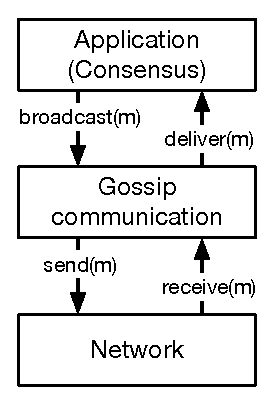
\includegraphics[width=0.3\columnwidth]{figures/modular.eps}
%\caption{Modular gossip design.}
%\label{fig:modular}
%\end{figure}

An algorithm interacts with the gossip communication layer using a {\em
broadcast} primitive that addresses a message to all \nodes. It is a
non-blocking primitive, as the dissemination is asynchronous and may take
several rounds.
The {\em deliver} primitive returns messages broadcast by \nodes. It is a
blocking primitive returning messages locally broadcast and messages received
from other \nodes.
%
There are no guarantees that a message broadcast by a non-faulty \node \ is
delivered by all non-faulty \nodes; due to other \node s'   failures, a
message may never reach some destinations.
In addition, the random choice of peers to which messages are sent may not
provide full connectivity.
However, a proper choice of parameters provides very high reliability,
specially when the {\em push} dissemination strategy is adopted \cite{Birman99}.
%\fd{I wonder if we need this discussion - on the other sied, we have space...}


\subsection{Tendermint}
\label{sec:Tendermint}

Tendermint \cite{buchman2019latestgossipbftconsensus} powers Cosmos, a network of proof-of-stake blockchains.
Both Tendermint and Cosmos are mature technologies, used by over a hundred businesses and running  on hundreds of computing nodes.
Tendermint builds an overlay network: a \node \ communicates directly with a restricted subset of \nodes, the node's neighbors or peers. 
To send a message to \nodes \ that are not its peers, a \node \ relies on gossip communication.

A \node \ is expected to maintain a long-term persistent identity in the form of a public key, from which the node's unique ID is derived. 
When attempting to connect to a peer \node, the first verifies whether the peer \node \ is in possession of the private key corresponding to its ID, thus preventing man-in-the-middle attacks. 
%To ensure liveness, 
We assume that each \node \  is connected to at least $f+1$ peer \nodes, ensuring that at least one of the connected \nodes \ is honest. 

%\nm{This does not guarantee liveness; to guarantee liveness, you need to have the f+1-connected network, meaning that even if $f$ Byzantine replicas stop participating,
%the network will remain connected, and honest replicas will be able to communicate. To ensure a $f+1$ connected graph, each node having at least $f+1$ peers is necessary but insufficient.}   %\fd{Indeed, we are not checking this. I just omitted liveness from this discussion above.  Any idea how to proceed?.}

Tendermint runs a sequence of consensus instances.
An instance is also called a height and decides one block of transactions.
To decide a height, one to multiple attempts, called rounds, can be needed.
%
Nodes play the role of \textit{proposers} in the first round of successive heights of consensus
according to a function \textit{proposer(height, round)} known by all nodes.
To handle asynchrony and failures, a new round in the same height can be initiated and led by a different node.
%
Nodes also have voting power to accept (or not) blocks being proposed, acting as \textit{validators}.

%Each round has a validator leader, the round's proposer, and coordinator.  
Similar to PBFT's execution \cite{CL99:osdi}, composed of three steps, 
a failure-free round in Tendermint has the steps \textit{propose, prevote} and \textit{precommit}, briefly explained below for node \textit{n}.

\fp{The following fragment needs editing, as it doesn't naturally follow the text before. It'd be good if Daniel could double check this.}  \fd{reviewed this.}

\begin{description}
\item[init] \textit{height=1, round=1};
\item[upon] \textit{n == proposer(height,round)}: 

broadcast PROPOSAL  with a signed block of transactions and identification $id$;

\item[upon] receiving \textsc{PROPOSAL} from the current height and round's proposer:  

if the block can be accepted, sign and broadcast \textsc{PREVOTE}.  

Acceptance depends on further consensus rules and validation by the application;

\item[upon] receiving \textsc{PROPOSAL} and matching \textsc{PREVOTE} messages from a quorum for the block $id$: 

broadcast a signed \textsc{PRECOMMIT} message for the block $id$;

\item[upon] receiving \textsc{PRECOMMIT} for the same block $id$ from a quorum: 

commit the block and append to the blockchain.  

 Deliver block's transactions to application and proceed to the next height, 1st round.  
\end{description}

Coherent with the proof-of-stake approach \cite{Poelstra2015DistributedCF}, nodes may have distinct voting power, that is, the vote of one node may have more weight than another.
A quorum is built by a subset of nodes aggregating more than $2/3$ of the total voting power.  

The straightforward description above is then enriched with additional rules to define whether a proposer must re-propose a block accepted in a previous round, and whether a node should accept the block proposed in a round.  The full algorithm can be found in \cite{buchman2019latestgossipbftconsensus}. 

%With equally distributed voting powers, this is the same as BFT quorums.   
%Validators with more voting power also become proportionally more frequent proposers.
% in the first round of new heights. 
%\nm{Do they become 
%proportionally more frequent proposers only in the first round of new heights or in general? I am not sure about this, but I think this is even true at the moment in Tendermint. } \fd{Not sure about this detail...  As we are not using this feature in the experiments, i just let the text generic in this regard.} 

The set of nodes is defined per consensus height.  The initial set is defined at the genesis state.  Then, modifications can be carried out with application commands.  The new set of nodes is proposed as an instance and is adopted if accepted.





%!TEX root =  report.tex
\section{Semantic Gossip}
\label{sec:semantic}

%\new
In this section, we first motivate investigating the interplay between consensus protocols and gossip communication. We then propose semantic gossip mechanisms, and elaborate on design details.

% motivation - in the Tendermint case - 
% what are situations where Tendermint's and gossip's redundancy could be reduced ?  ...
% concrete situations where communication could be spared.   unneeded (motivate filtering), optimisations possible  (motivate aggregation)

% design -

% layering

% semantic filtering 

% semantic aggregation

% implementation

% motivate the need for gossip protocols optimized for consensus, 
% describe the design of a gossip protocol that takes advantage of consensus semantics, 
% and detail its implementation.



\subsection{Motivation}
\label{sec:motivation}

Using gossip as a communication layer for consensus is in general a straigthforward adaptation:
the direct point-to-point communication using a set of channels providing full connectivity
is replaced by gossip a layer that reaches all processes.  
%
One of the reasons it is straightforward is because the consensus layer deals with process failures and communication problems that may arise, which makes it robust  to be used with different underlying communication properties.    
%The Tendermint protocol uses gossip for interprocess communication.  

In the following we discuss two fundamental characteristics of a wide range of consensus protocols
that motivate the investigation of the interplay of consensus with a gossip communication layer.

\subsubsection{Detecting quorums}
\label{redundant}

%generic
One way to design redundant systems is through the concept of quorums.
A quourum can be understood as a level of redundancy sufficient to allow the protocol to progress while keeping safety, under the fault model assumption.    
%When a node gathered matching messages from a quorum of nodes, further messages belonging to the same step are typically ignored at the node, i.e. redundant.
%generic
Considering this, a node could spare to send messages if it already knows a quorum has been
achieved by other nodes.
While this observation does not help when nodes communicate directly,
%
%Using point-to-point communication this approach is not natural, if not impossible to explore since this would mean that a node would await a quourum to be built to spare sending a messsage that should contribute to that quorum - a contradiction.    
%
%However, 
the use of gossip at the communication level allows to benefit from it.  
If a node receives a message $m$ and computes that it already has matching messages from a quorum of nodes, it assumes the previous messages, sufficient to build a quorum, were forwarded.  Thus the redundant message $m$ (and further ones) is not needed at the neighbour nodes and is not forwarded.
This redundancy elimination is however only possible if the gossip layer is aware of the consensus protocol semantics.

\subsubsection{Phased communication}
\label{obsolete}
%generic
Consensus protocols are typically organized in communication instances, and proceed in rounds using corresponding message types.
This helps to detect if a given message is obsolete for the current progress of the protocol. %  It could have been delayed or originated by a late node, and is no longer valid. 
In such case it could be ignored.
%
A further observation is that,
as nodes behave simmetrically, 
it is common that the same types of messages, stemming from different nodes are communicated concurrently through the network.
%
While using direct communication this maybe a pointless observation,
when using gossip we can unfold the examination:
messages with the same semantics, but differing in the specific node's
answers (e.g. votes), will coexist in intermediate nodes along the gossip forwarding.
Moreover, it is typical that such messages are addressed to the same set of nodes (all that participate in the consensus protocol).  
In such cases, instead of forwarding and processing separately each such message, they can be aggregated at an intermediate node, 
resulting one message collecting the space of parameters of the equivalent bunch of messages.
This leads to sparing both messages through the network as also message processing at destinations. 

\old

\subsection{Design}
\label{sec:design}

In this section, we discuss simple techniques to address the mismatch between a
fault-tolerant consensus algorithm, using Tendermint as reference, and the
underlying gossip communication substrate.
The goal is to reduce the message redundancy at the gossip layer,
employing the knowledge about the message semantics provided by the
consensus algorithm.
The challenge is to achieve this reduction in message redundancy without sacrificing
(a) modularity, (b) consensus properties, and (c) the original resilience guarantees offered by gossip. 

\subsubsection{Semantic filtering}

The first technique allows the consensus algorithm to decide whether a message should be sent to other nodes at the gossip layer.
%This means interferring with the operation of the gossip layer, which, by default, forwards every message received.
The consensus algorithm can then restrain the propagation of messages that are (potentially) no longer useful to other nodes.
%The main goal is to save network and processing resources that would be used to forward messages that peers will probably disregard.
Semantic filtering is implemented through a set of rules to identify messages that, according to the consensus semantics, have become redundant or obsolete, as discussed in Sections \ref{redundant} and \ref{obsolete}.
%
The semantic filtering rules are evaluated when a message is ready to be sent to peer nodes.
If the message is filtered out, because it is identified as either obsolete or redundant, the gossip layer discards it; otherwise, it is sent as usual.

The evaluation of the semantic filtering rules can be seen as a lightweight
execution of the consensus algorithm on behalf of another node.
In fact, to identify messages that can be filtered out it is necessary to store
some information about messages that were previously sent to other nodes.
The more comprehensive the rules are, the more information is stored per peer node,
and the more costly it is to evaluate them.
Thus, the choice of a set of semantic filtering rules should balance the cost
of evaluating them for every message forwarded, with the benefits that an
effective filtering can provide.

\paragraph{Semantic filtering in Tendermint} 
As discussed  in Section \ref{sec:Tendermint}, a node progresses   to the next step when a quorum of \textsc{prevote} or \textsc{precommit} matching messages is received.  Additional messages of these types are not needed.  Also, duplicted messages are not usefull and need not to be forwarded.   The filtering rules thus state that a vote message is dropped by a node in the following cases:  
\begin{itemize}
\item If a vote of the same type (either \textsc{prevote} or \textsc{precommit}), with the same originator,  height, round, and value has been already computed before by the node;
\item If the vote (either \textsc{prevote} or \textsc{precommit}) is for a height and round for which the node has already handled a quorum of matching votes.
\end{itemize}

\paragraph{Semantic filtering keeps consensus properties}

Discarding messages at the gossip level is perceived as message loss (absence of) at the consensus level.  Thus, filtering could at most prevent progress but not safety.
To ensure progress, a filtering mechanism cannot hinder nodes from receiving messages from a quorum. 
%
Notice that with the first filtering rule the message dropped has been handled before and
with the second filtering rule, a node discards messages after having handled a quorum of matching messages.   In both cases, since the node handled the previous messages, they were already forwarded via gossip to other nodes.  

\fp{The text here is unclear, as the message already could be lost.}

\fp{What does it mean for ``a quoru to be identified at a node''?}  

%In such case, the node already forwarded a quorum of messages to its neighbours that, therefore, already have votes to build a quorum too. Again, the current message is not needed.

\subsubsection{Semantic aggregation}

The second technique provides the consensus algorithm with the possibility to
replace a number of similar or related messages, which will be sent to a peer,
with a single message comprising the information carried by the original
messages.
This technique explores the scenario in which the gossip layer has multiple
pending messages to send to a peer, so that some of them are likely, according
with the consensus semantics, to be aggregated.
It is an opportunistic mechanism that aims to reduce the number of messages
exchanged by processes via gossip, especially when they operate under moderate
to high load.

Semantic aggregation is also implemented through a set of rules that, from a
list of pending messages: (i) identify those that are prone to aggregation, and
(ii) define how an aggregated message can be built from the original messages.
When messages prone to aggregation are found, the first of them in the list of
pending messages is replaced by the aggregated message, built according to
the respective rule, while the remaining ones are removed from the list.
In other words, an aggregated message both replaces and filters out the
original messages that it aggregates.
Messages that are not prone to aggregation, or for which aggregation is not
deemed advantageous by the consensus algorithm, are not affected by this
technique.
They are kept in the list of pending messages, and are forwarded to the peers as
usual.

Semantic aggregation rules can be either reversible or not.
When a process receives from a peer a message aggregated using a reversible
rule, it reconstructs the original messages and treats them as regular messages.
That is, messages received for the first time are delivered to the
consensus algorithm and forwarded to other peers.
In this process, in
particular, they can be semantically aggregated again.
When an aggregated message is built from a non-reversible rule, it is treated
as a new message broadcast by the process that aggregated it.
In this case, the consensus algorithm must be able to handle the
semantically aggregated message.

Observe that, despite the similarities, semantic aggregation is not the same as
batching~\cite{FR95}.
When implemented at network level, batching essentially concatenates messages,
treated as raw byte arrays, to optimize the network usage.
At application level, some message types are batched until the batch size
reaches a threshold or a timeout expires.
As a result, batching can have negative effect on performance when the system
is subject to low loads, as the sending of messages is postponed.
This does not happen with semantic aggregation, which despite being ineffective
under low loads, does not delay the sending of any messages.
Moreover, the technique is more flexible than batching, as messages are not
only concatenated, but can be transformed, merged, in any arbitrary way defined
by semantic aggregation rules.

\paragraph{Semantic aggregation in Tendermint}

Regarding Tendermint, semantic aggregation is also applied to 
\textsc{prevote} and \textsc{precommit} voting messages.
Given a subset of messages to be sent to a peer, messages of the same type (\textsc{prevote} or \textsc{precommit}), for the same height, round and value (block id) can be aggregated.
The aggregated message carries a list of pairs $\langle origin, signature \rangle$ identifying originators of the  messages aggregated, and only once the identical contents.

\paragraph{Semantic aggregation keeps consensus properties}

The basic requirement for a sound aggregation strategy is that the information conveyed by an aggregated message is equivalent to the original non-aggregated ones, enabling the same decisions to be taken at the destination.
%
%Observe that the aggregation rule proposed for Tendermint does not exclude information, only data.\fp{I don't get this. What's the difference between information and data?}

Notice that the restriction to aggregation is strong: aggregated messages should be identical, only stemming from different originators.   
%
The receiver of the aggregated message, be it \textsc{prevote} or \textsc{precommit}, will compute the exact same votes as for the non-aggregated messages.
%
%A strong aggregation restriction makes it easier to show sound and, although it may seem less effective, as consensus protocols often use communication phases with same message types sent among processes, aggregation shows important benefits, as discussed further in the paper.\fp{Convoluted sentence...}

\subsubsection{Semantic Gossip and BFT}

To ensure that aggregation and filtering are not exploited by dishonest nodes,\footnote{For example, a dishonest node could forge messages to exploit the proposed mechanisms.  Consider a dishonest node $dh$ that forges a \textsc{prevote} message for a given height and round, pretending to be node $a$, and sends it to node $b$.  Since gossip does not verify messages, $b$ would record $dh$'s message and on the occasion of the original message from $a$, it would be filtered out with the effect of possibly preventing progress.} 
we ensure that any message is verified before the respective decisions are made by Semantic Gossip. \fp{I don't get this part.}




From an engineering perspective, as signature verification is one of the first measures taken at the consensus layer to avoid attacks, and being a costly procedure, instead of performing verification additionally at the gossip layer we propose an interface to return a copy of delivered and verified messages to the gossip layer.   With this, gossip can further handle the message without increasing the overall overhead.
This aspect is shown in Figure \ref{fig:architecture_sg} with the loop-back arch from signature verification at consensus to the filtering input queue at the semantic gossip layer.

%\fd{argue this is enough to handle bizantine processes ?}

%Semantic Gossip adopts that  Filtering and Aggregation decisions should be taken also based on verified messages.  


\subsection{Implementation}
\label{sec:impl}

%\color{violet}

We implemented a gossip-based communication layer to interconnect processes.
At the system setup, each process opens connections to a randomly selected set
of processes.  The resulting overlay has to be connected and each node is required to have at least $k=f+1$ neighbours.
Section \ref{sec:topos} discusses how nodes can create such an overlay using a distributed procedure.


\subsubsection{Classic gossip}

Figure~\ref{fig:architecture} (left) illustrates the architecture of a gossip layer.
A process interacts with the gossip layer through primitives {\em broadcast} and {\em deliver}.   Broadcast messages are handled just as gossip messages received from other peers.   Messages are delivered once they pass the duplication check.
The {\em delivery queue} offers messages to the upper layer.

A process also maintains, for each peer it is connected to, a Send and a
Receive routine. A {\em send queue} is associated to each Send routine; messages added to a {\em send queue} are eventually sent to the corresponding peer.
%There is a single {\em  receive queue} shared by 
All Receive routines share the same queue with the local broadcast.  
%
A message added to the {\em broadcast and delivered queues} is locally delivered and sent to
all peers but the peer the message came from: it is added to the {\em delivery
queue} and to all, but the message's origin, {\em send queue}s.
%
The selection of peers to which a message is sent is done by the message
forwarding module from the gossip main routine.    

%% Controlling the flood via recently seen cache
Messages are propagated using the {\em push} disseminating strategy. 
This means that the same message can be received by a
process several times, from distinct peers.
%
We control the flooding of messages using a simple approach based on a cache of recently received messages, maintained by every process.
%
A message is registered to the recently received cache before it is delivered
to the consensus algorithm and sent to the process' peers.
If the same message is received within a short period of time, so that the message's
identifier is still on the recently received cache, the message is
dropped---i.e., it is not delivered nor forwarded to the peers.
%
This is the role of the duplication check module represented in
Figure~\ref{fig:architecture}: it prevents, with some probability, a message
from being delivered and forwarded more than once. 
%
There is no actual guarantee of a deliver-and-forward once behavior, but the
adoption of a reasonable cache size reduces the probability
of message duplication.
%
It is worth noting that the cache stores message identifiers (hashes), not full messages, and so, it is relatively small.

\subsubsection{Semantic extensions}

The gossip layer offers two ways to control its behavior: semantic filtering and semantic aggregation, as presented in Section~\ref{sec:design}.
The consensus algorithm can adopt one or both techniques by implementing interface methods offered by the gossip layer.   
Figure \ref{fig:architecture_sg} (right) depicts how the classic gossip architecture is extended for filtering and aggregation, and identifies which functions are needed from the consensus layer, i.e., encapsulating semantics of the specific consensus protocol.

\begin{figure*}[htbp]
    \centering
    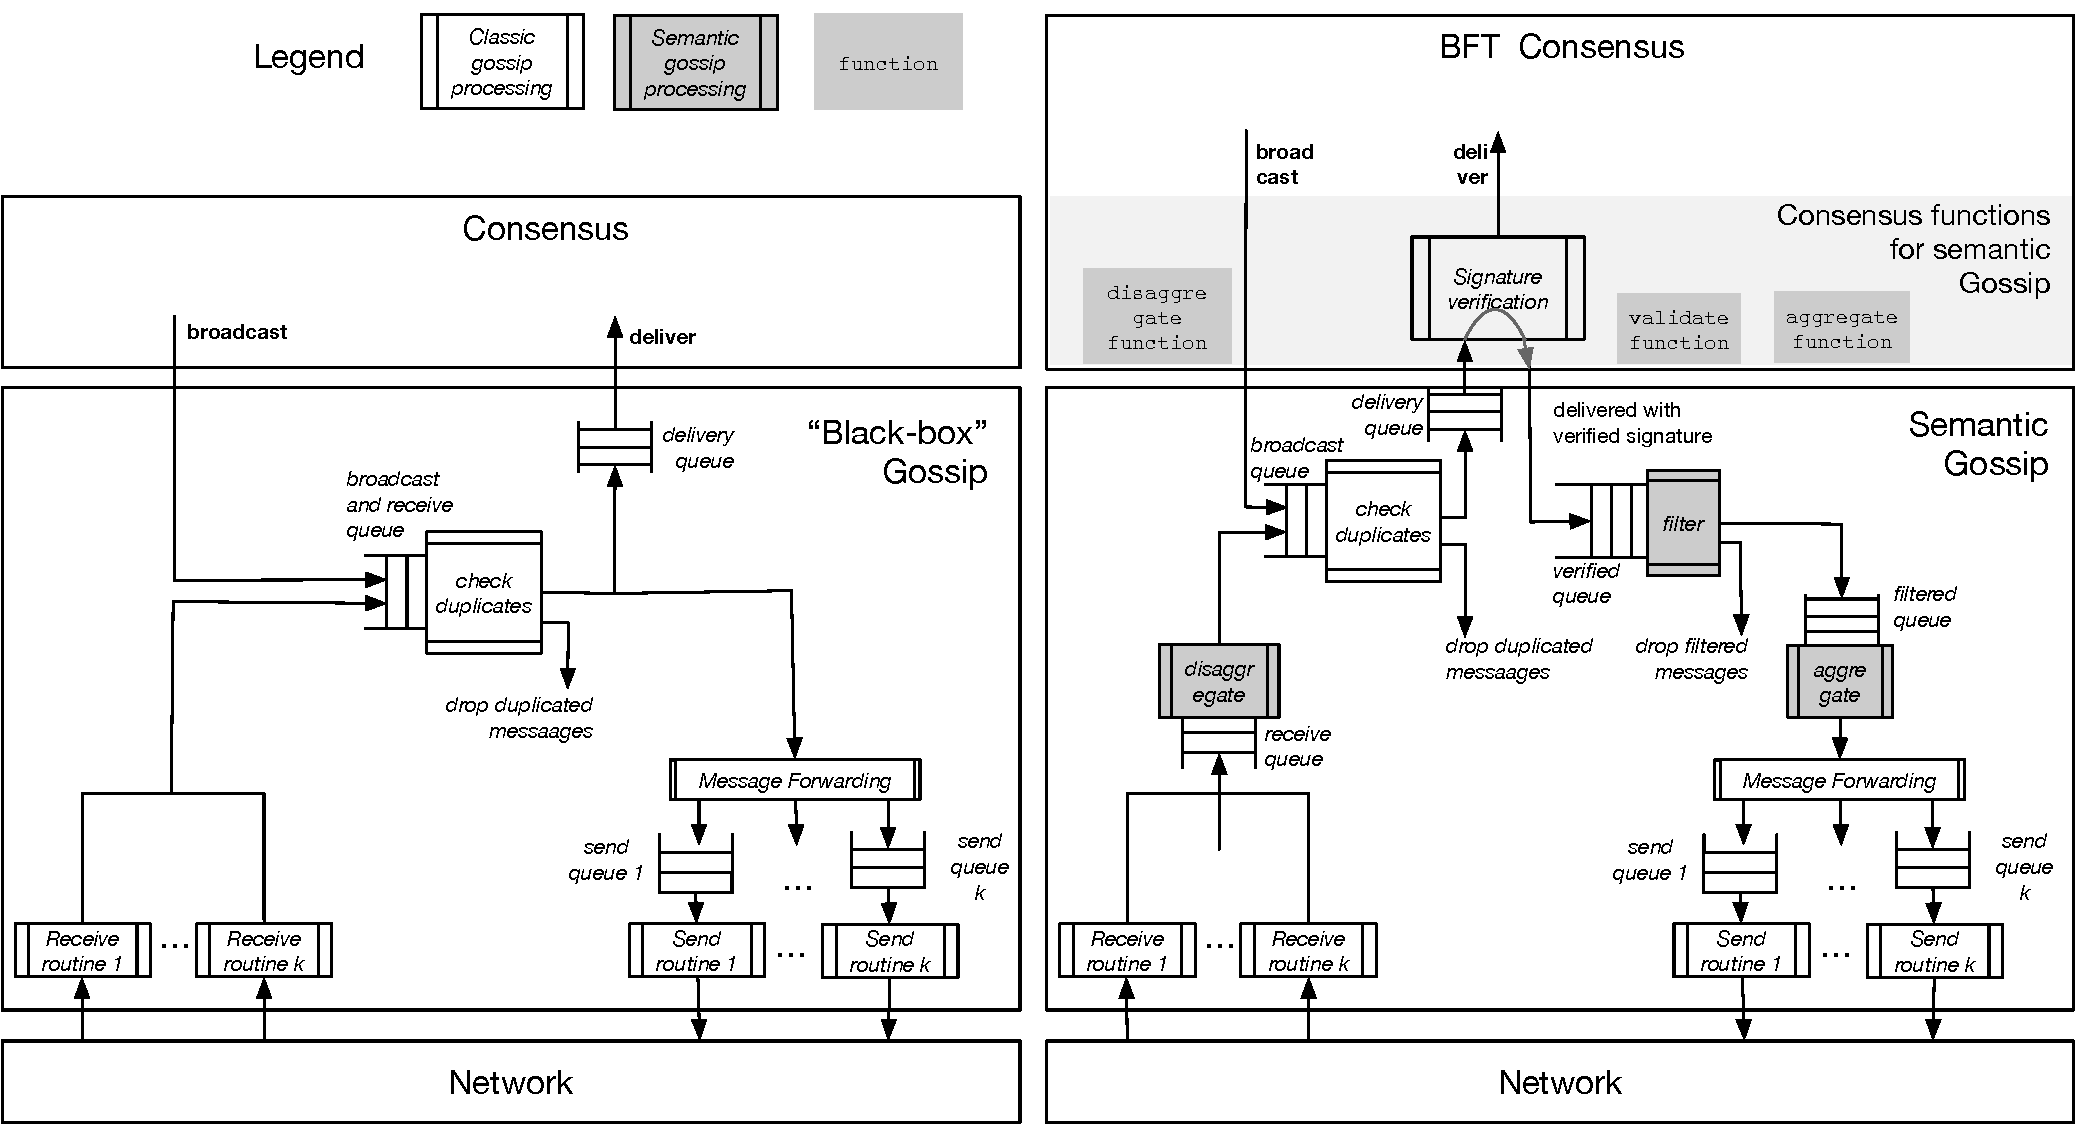
\includegraphics[width=1\columnwidth]{figures/architecture_SG3.pdf}

    
    \caption{Architectures: (left) - Gossip;  (right) Semantic Gossip}
    \label{fig:architecture}
    \label{fig:architecture_sg}
\vspace{-2mm}
\end{figure*}
% \begin{figure}[htbp]
%     \centering
%     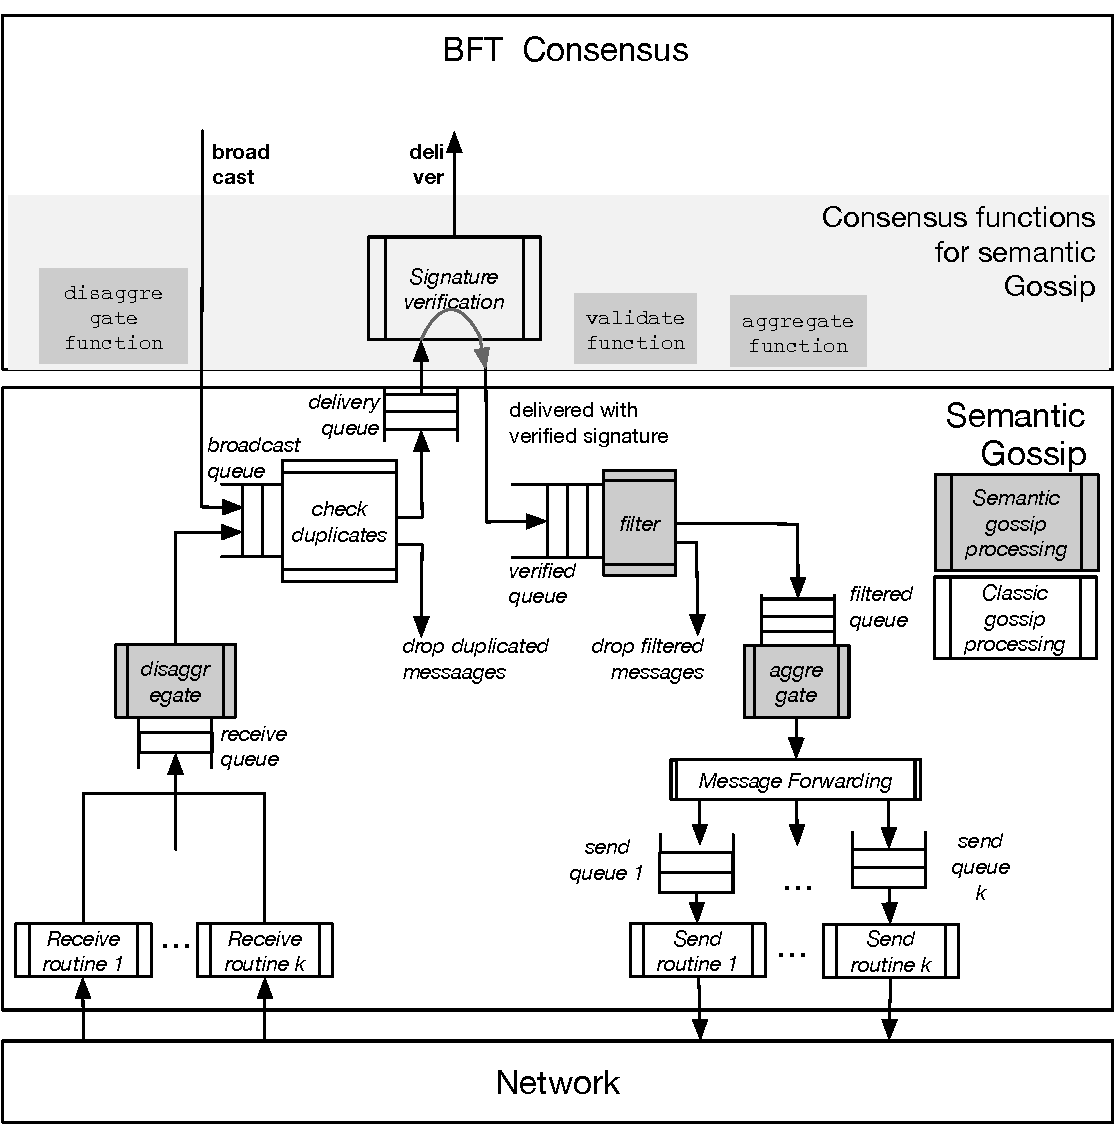
\includegraphics[width=1\columnwidth]{figures/architecture_SG2.pdf}
%     \caption{Architecture of semantic gossip at a process.}

% \end{figure}

\paragraph{Semantic filtering} is provided by allowing the consensus algorithm to implement
a {\em validate} function, which receives a message and a destination peer, and
returns a boolean:

\begin{verbatim}
Bool validate(Message, Peer)
\end{verbatim}
The {\em validate} function is invoked by the {\em filter} module at the gossip layer when a message has not been dropped due to duplicates or signature violation, and is considered for forwarding.
%
If the function returns false, the message is dropped, as the decision was to
filter out the message.
Otherwise, the message is sent to the peer, the default behavior when the
function is not implemented.
%
Implementations of the {\em validate} function should be fast and non-blocking,
as it is likely to be invoked concurrently by multiple sending routines.
The implementation should keep some information about the state of each peer,
essentially a summary of relevant messages that were previously processed and
not filtered out, and thus sent to that peer.
The cost of storing such information versus the benefit in terms of resources
saving by filtering out messages that would be sent to a peer
should be considered.


\paragraph{Semantic aggregation} is provided through the implementation of a pair of
functions, {\em aggregate} and {\em disaggregate}, by the consensus layer:

\begin{verbatim}
Message[] aggregate(Message[], Peer)
Message[] disaggregate(Message)
\end{verbatim}

The {\em aggregate} function receives an array of messages and a destination
peer, and returns an array of messages.
It is invoked by the gossip {\em aggregate} module when there are multiple pending messages to be sent to the respective peer.
%
%\fd{AGGRETATION APPLIES TO DIFFERENT KINDS OF MESSAGES, TO THE SAME DESTINATION ?  OR ALL CONSTITUTENS OF AN AGGREGATED MESSAGE ARE OF THE SAME TYPE?}
%
Messages returned by the {\em aggregate} method, either original untouched or 
aggregated, are sent to the peer, in the order in which they are returned.

Any message received from peers can be aggregated.  
The {\em disaggregate} module at the gossip layer invokes the 
the {\em disaggregate} function provided by the consensus layer when a message marked as
aggregated is received.
The {\em disaggregate} function 
is the inverse of {\em aggregate}: it receives an aggregated message and returns an array of reconstructed messages, for reversible semantically aggregated
messages.
Messages returned by the method are processed as regular messages, in the order
in which they are returned.
These messages are checked against the recently received
cache and, if not duplicated, delivered and forwarded to peers.




%!TEX root=report.tex
\new
\section{Experimental evaluation}
\label{experiments}

Having proposed and argued for the semantic gossip mechanisms, we addressed the first research question defined in Section \ref{sec:intro}.   Now, we turn our attention to the 
sencond and third research questions.  To address those we build a prototype of our ideas and conduct a series of experiments.

%we want to evaluate their effectiveness. % We aim at a better performing consensus protocol with the same resilience.  
%We conduct experiments to give answer to the sencond and third research questions defined in Section \ref{sec:intro}.
%following main questions:
%\begin{itemize}
%\item is there a gain in performance of consensus, and how much, using each of the mechanisms, and combined, in relation to none ?
%\item is the vulnerability of consensus increased in the presence of increasing number of dishonest nodes ?
%\item \fd{is that all?}
%\end{itemize}

\subsection{Methodology}
\label{ref:method}

Gossip networks are typically built having nodes connecting to a number of randomly chosen peers.
A basic concern is how different topologies 
could affect gossip and the proposed mechanisms and thus impact the consensus protocol using gossip.   To address this concern, our study starts with a characterization of possible topologies obtained from a gossip arrangement of nodes, and their properties, in Section \ref{sec:topos}.
%
We then present system configurations and deployments to conduct experiments in Section \ref{sec:setup}.
%Using a class of representative topologies with the system configurations described we conduct experiments aiming to answer the above mentioned questions.
%\fd{review}
The first set of experiments aims to answer the second research question, being
reported in Sections \ref{sec:overall} to \ref{sec:latency-cdfs}. 
We used increasing workload 
aiming to assess the relation of throughput and latency.
The workload is increased by stepwise enabling Tendermint to handle more 
instances concurrently.
%\fd{review}
Regarding the third research question, resilience evaluation is reported Section \ref{sec:resilience}.  
We fixed a workload and assessed resiliency by 
stepwise increasing the number of byzantine nodes in the network from 0\% to 30\%, 5 by 5\%.   For each case, we observe again the result of throughput and latency.
In Section \ref{sec:msgLoss} we evaluate throughput and latency under increasing message loss rate.

%Finally, we additionally report on the observed impact of signatures validation needed in the semantic layer, in Section \ref{sec:signatureImpact}.
%\fd{DO WE ?}















\subsection{Choice and Distributed Generation or Network Overlays}
\label{sec:topos}

Due to the random generation of network overlays by the gossip protocol, 
we have to ensure that the overlays used in the experiments are representative, not leading to distortion in the measures obtained.
Moreover, we have to provide a distributed algorithm to generate these overlays. In this section we discuss how the overlays used in the experiments can be obtained and their characteristics.

\subsubsection{Network overlay definition}

A network overlay is a graph $G(V,E)$, where $V$ represents the set of
processes running the experiment (validator nodes) and $E: V \times V$ represents the set of bi-directional network connections between processes.  $G$ is simple (a process does not connect to itself and there is only one edge among any two nodes) and non-directed
(an edge means communication in both directions is possible).  The following definitions are useful in next sections:
\begin{itemize}
	\item $peers_G(p \in V) := \{q \in V : (p, q) \in E\}$ is the set of processes directly
	connected to $p$ in the overlay $G$.
    \item $degree_G(p \in V) := |peers_G(p)|$ is the number of connections process $p$ has in
  the network overlay $G$.
   \item   $outPeers_G(p \in V)$ and $inPeers_G(p)$: the set of outbound and inbound peers of $p$, i.e., 
	processes $q \in peers_G(p)$ to which $p$ is expected to respectively dial
     and establish a connection, or accept a connection request.
\end{itemize}

\paragraph{Soundness} A network overlay is valid, said sound, if the following requirements are fulfilled:
\begin{itemize}
\item connected: $G$ is connected, i.e., there is a path
built out of edges in $E$ among any two processes in $G$.
\item minimum neighbourhood: for fault-tolerance,  each node in 
the overlay is required to have
at least $f+1$ neighbours, where $f$ is the allowed number of faulty processes,
ensuring that any node is always connected to at least one honest node.
In our case $f < n/3$, $n$ being the total number of nodes.
\end{itemize}

% For any two processes $\{p, q\} \in V$, if $(p, q) \in E$ then there is a 
% connection between processes $p$ and $q$ in the network overlay $G$.
%In order to properly model the behavior of the network, a network overlay $G$
% has the following properties:   
% \begin{itemize}
% 	\item $G$ is a simple graph, i.e., $(p, q) \in E \implies q \neq p$, as processes
%   do not connect to themselves;
%     \item  $G$ is a undirected graph, i.e., $(p, q) \in E \implies (q, p) \in E$,
%   as connections are bi-directional.
% \end{itemize}
%

%On a more specific terms, it is interesting if the process $p$ is able to
%classify its peers in two categories:
% UNNEDED:  Also, $outPeers_G(p) \cup inPeers_G(p) = peers_G(p)$ and 
% $outPeers_G(p) \cap inPeers_G(p) = \emptyset$.
% The classification of peers in outbound or inbound peers is antisymmetric:
% $\forall p,q \in V$ if $q \in outPeers_G(p)$ then $p \in inPeers_G(q)$.
% In practical terms, this means that process $p$ will dial process $q$,
%while $q$ will not dial process $p$, but wait for a connection request from it.
%## Random overlays

%Since there is a large amount of possible network overlays for a given 
%set of processes, we produce and analyze randomly generated network overlays.

\subsubsection{Distributed generation}
\label{sec:distributedGeneration}

Given a network overlay $G$ to be used in an experiment (or instantiation of
the protocol), each process $p \in V$ should be able to compute the 
set $peers_G(p)$ with which they should be connected in the adopted network overlay.
Each process $p$ has to be able to identify its $in$ and $outPeers_G(p)$.
%
%\subsubsection{Network overlay characterization}
For its generation, we characterize a random network overlay using three parameters:
\begin{itemize}
	\item  $n$: the number of processes in the network, i.e., $n = |V|$.
    \item  $k$: the connectivity parameter, which can be seen as the target value for
  $degree_G(p)$ for every $v \in V$.
    \item $s$: the seed employed to randomly select the connections between processes
  in the network overlay.
\end{itemize}

Notice that $n$ and $k$ are parameters for the generation of a class of random
network overlays, while $s$ allows to uniquely identify each individual random
network overlay belonging to that class.   
%
Using the same seed and random number generator, a deterministic distributed algorithm can be used to compute the same network at each distributed process. In a distributed algorithm, if each of the $n$ nodes chooses $x$ neighbours to connect, the expected final number of neighbours of a node\footnote{$E_{nbr} = A + B - C$ where: $A$ is the number of neighbours chosen by this node, $A=x$; $B$ is the number of nodes that choose this one has neighbour, as $n$ nodes choose this one with probability $x/n$, $B=n \times x/n$; and $C$ is the number of mutual choices that may take place, as two nodes choose to be neighbours with probability $(x/n)^2$, we have that for $n$ nodes $C = (x/n)^2 \times n$.   With this, $E_{nbr} = x + n \times x/n - (x/n)^2 \times n = 2 x - x^2/n$}
is $E_{nbr} = 2 x - x^2/n$.
%resulting graph $G$ will have average $degree_G$
%
%For example, in a network with $n=128$, since $f \leq n/3$ and $k\geq f+1$ each node should have at least $k=43$ neighbours. If each node independently chooses $k$ neighbours, the expected average $degree_G$ of nodes is $E_{nbr}=71.5$.
%To minimize the extra redundancy of the resulting overlays,
%we refine the simple approach above such that each node chooses
%$k'$ other nodes, and
To generate networks in which $E_{nbr}$ approaches the desired connectivity $k$, %where nodes have in average $k$ neighbours.
%each node has with $E_{nbr}$ approximating $k$.
%i.e. $k = n \pm \sqrt{n^2-n k'}$. Thus,
in the distributed algorithm we use $x$ obtained from the above relation. 
%, where 
%%%%%%  >>  $x =\lceil n - \sqrt{n^2-n k} \rceil$.
%we used $k' = n \pm \sqrt{n^2-n k}$.  As for $1 \leq k \leq n$, $(n + \sqrt{n^2-n k}) \geq n$,
%we take $k' = n - \sqrt{n^2-n k}$. % resulting in $0< k'\leq n$.
For instance, in a network with $n=128$, if we want nodes to have in average $k = 43$ neighbours, $x$ should be $23,69$. So we use $x = 24$: each node chooses randomly $24$ neighbours. 

Our deterministic algorithm for distributed overlay generation has the following main parts: assuming input $\langle k, n, seed \rangle$ and using the same random generator: (a) from $k,n$ find $x$ as above; (b) in the same order of nodes in $n$, for each node randomly choose $x$ neighbours; (c) if the network is not connected or there exists any node with less than $k=f+1$ neighbours, repeat from (b), otherwise adopt the network.  
To ease the process of finding a network with the needed minimum connectivity we can slightly increase $x$.

\paragraph{Classification}

\begin{figure}[htbp]
	\centering
	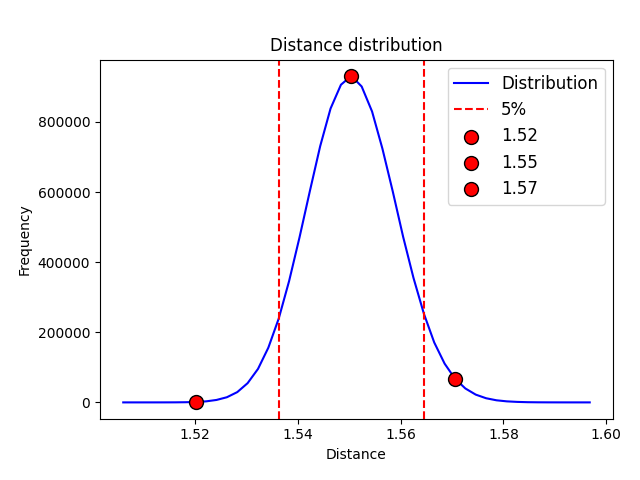
\includegraphics[%width=\columnwidth,
  height=5cm]{figures/n32-topology-distance-distribution.png}
	\caption{Distance distribution of the random generated overlays for n=32,k=13.8.}
	\label{fig:topologyDistribution}
\end{figure}

\begin{figure}[htbp]
	\centering  
	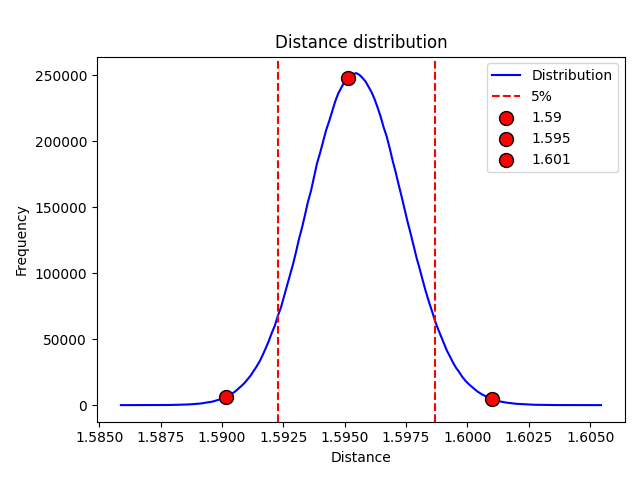
\includegraphics[%width=\columnwidth, 
     height=5cm]{figures/n128-topology-distance-distribution.png}
	\caption{Distance distribution of the random generated overlays for n=128,k=51.3 }
	\label{fig:topologyDistribution128}
\end{figure}

Once we have a distributed generation algorithm, we have to evaluate if radom generated topologies are free from any bias that may impact the results.
Since the distance among nodes is a fundamental aspect of gossip performance,  we classify overlays using their average shortest path length among any pair of nodes.  We call this metric the distance of an overlay and in Figures \ref{fig:topologyDistribution} and
\ref{fig:topologyDistribution128}
we present the distance distribution for overlays with $n=32$, $x=8$ leading to $k=13.87$; and $n=128$, $x=29$ leading to $k =51.43$.
%With this, we generate a population of sound overlays and, for each one we compute its distance, associating the triple $\langle k, n, seed \rangle$ to the value obtained.   After this,
We select sound instances from this population that are in different extremes of the distance distribution (below 5\% and above 95\%), as well as samples in the center of the distribution.  Experiments are run with each selected overlay instance, showing in Figures \ref{fig:n32TopologyComparison} and  \ref{fig:n128TopologyComparison} that they have comparable impact on all semantic gossip techniques, meaning that the techniques are not favored by the choice of different   topologies generated with the same arguments.  %\fd{TO DO:  In each fig we have to choose if we show the upper or lower part.   And then reshape it to become readable (font size in axes, legends, ...). The lower part shows more directly that the semantic gossip mechanisms are not impacted by different topologies in the distance distribution - for same conectivity parameter.}
%
Once this is observed, we follow the studies with the average distance topology (center of distribution).

%Each selected instance is used to configure a set of Tendermint validator nodes, these validators compute the same topology with the refined algorithm above, build the network connections, run the same workload, and extract performance metrics.  
%Experiments show that 
%showing equivalent results. Which leads to conclude that that the random generation of sound overlay networks with same parameters $\langle k, n \rangle$ lends networks with equivalent performance.

%\begin{figure*}[htbp]
%	\centering
%	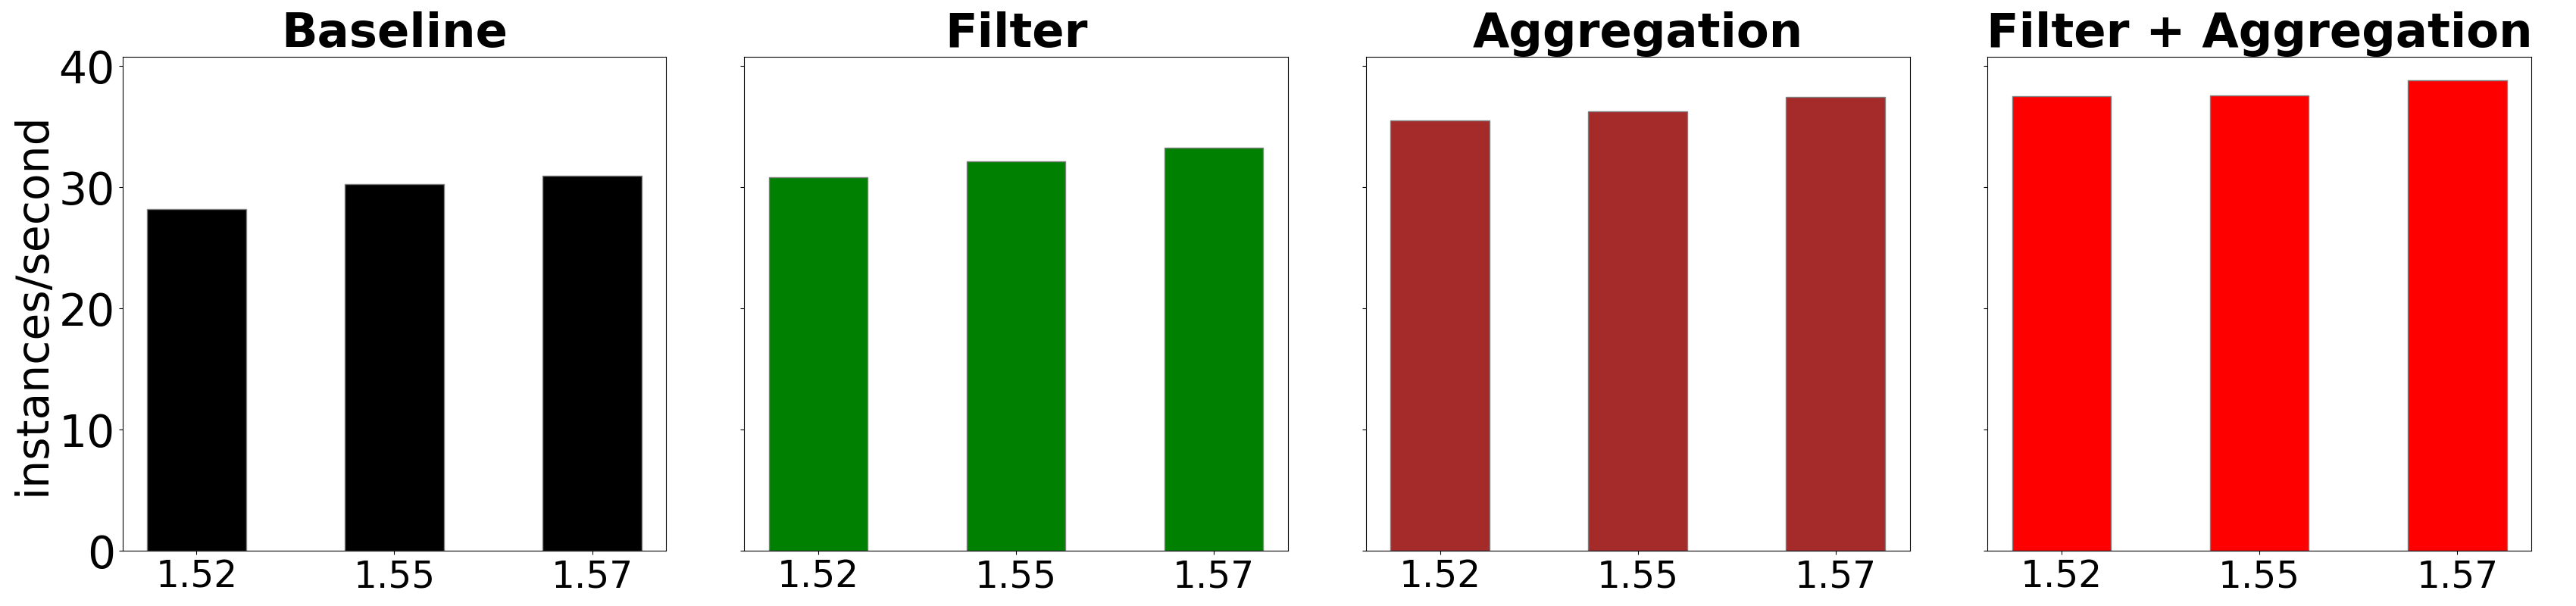
\includegraphics[
 %      height=3.5cm]{figures/topo-thr-hist-32n.png}
%	\caption{Throughput of the best throughput/latency relation points, for different setups and different average node distances (x axis for each setup) in a network with n=32 and k=13,8.}
%	\label{fig:n32TopologyThrComparison}
%\end{figure*}


\begin{figure*}[htbp]
	\centering

	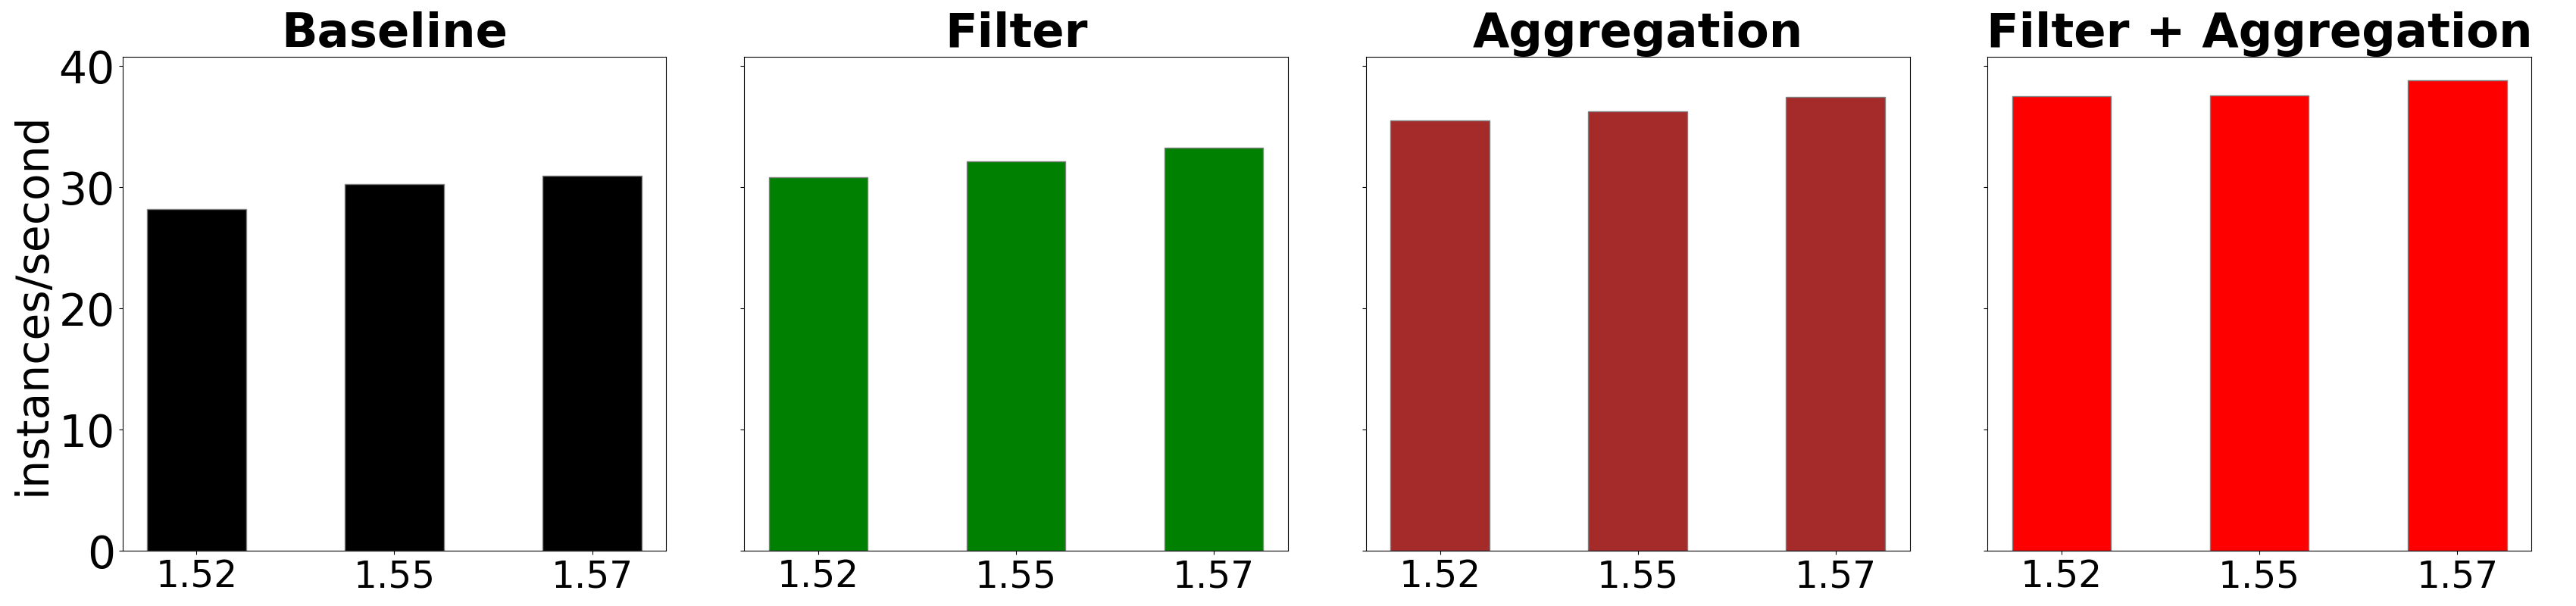
\includegraphics[
       height=3.5cm]{figures/topo-thr-hist-32n.png}

\vspace{5mm}

	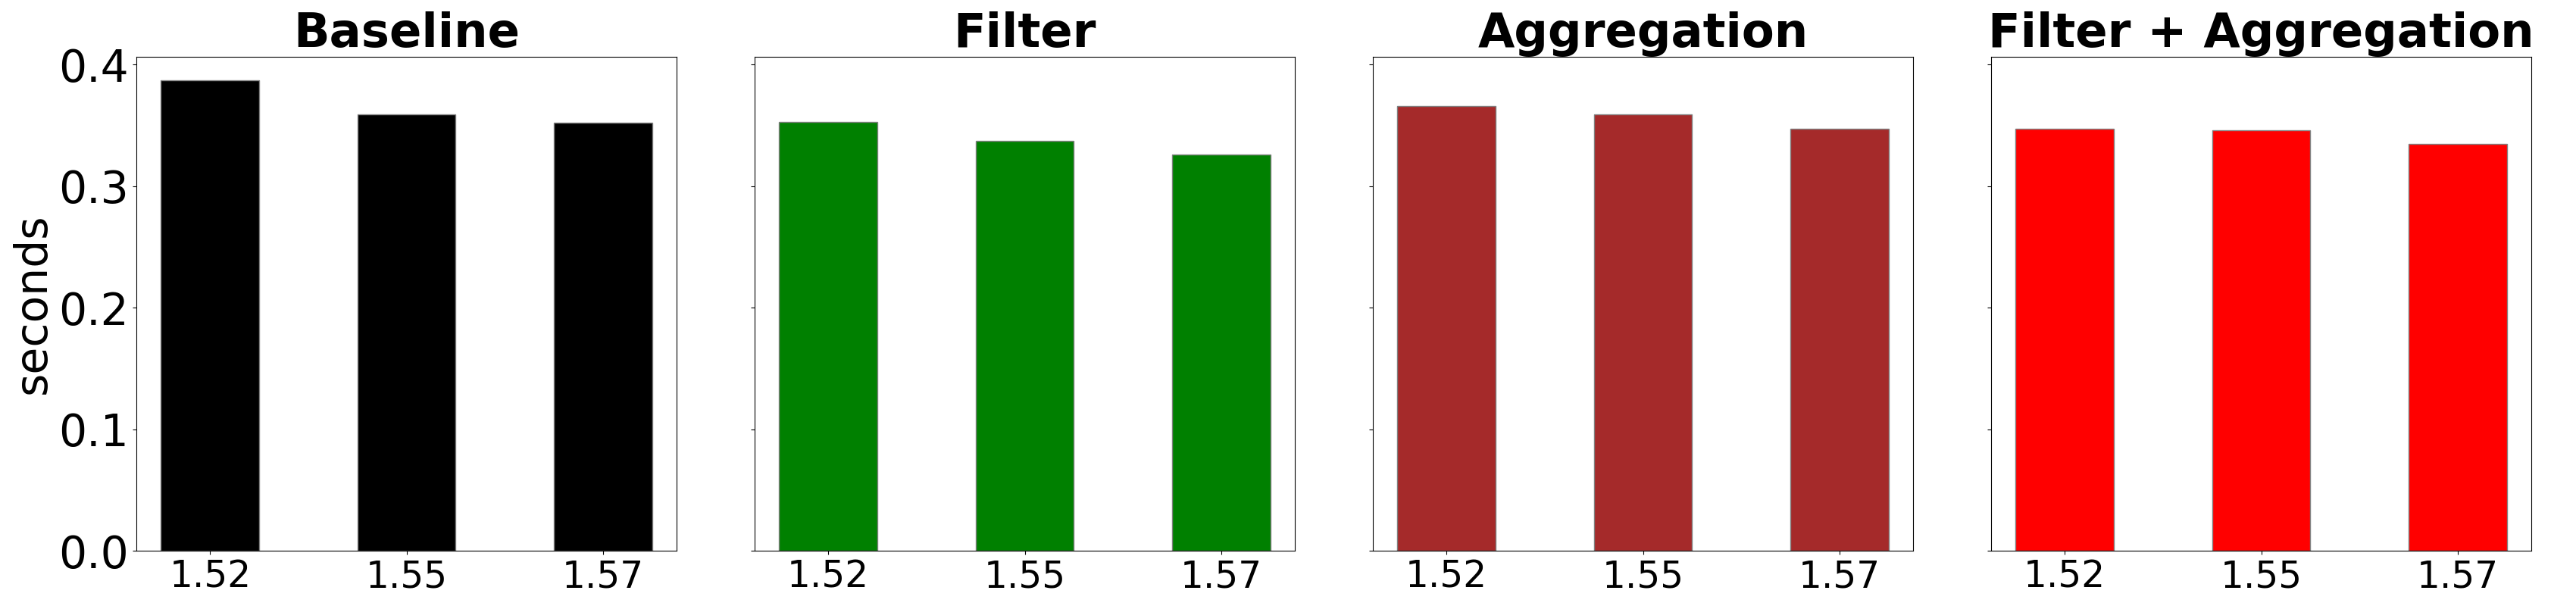
\includegraphics[height=3.5cm]{figures/topo-lat-hist-32n.png}
	\caption{Throughput (above) and latency (below) of the best throughput/latency relation points, for different setups and different average node distances (x axis for each setup) in a network with n=32 and k=13,8.}
	\label{fig:n32TopologyComparison}
\end{figure*}

\begin{figure*}[htbp]
	\centering
	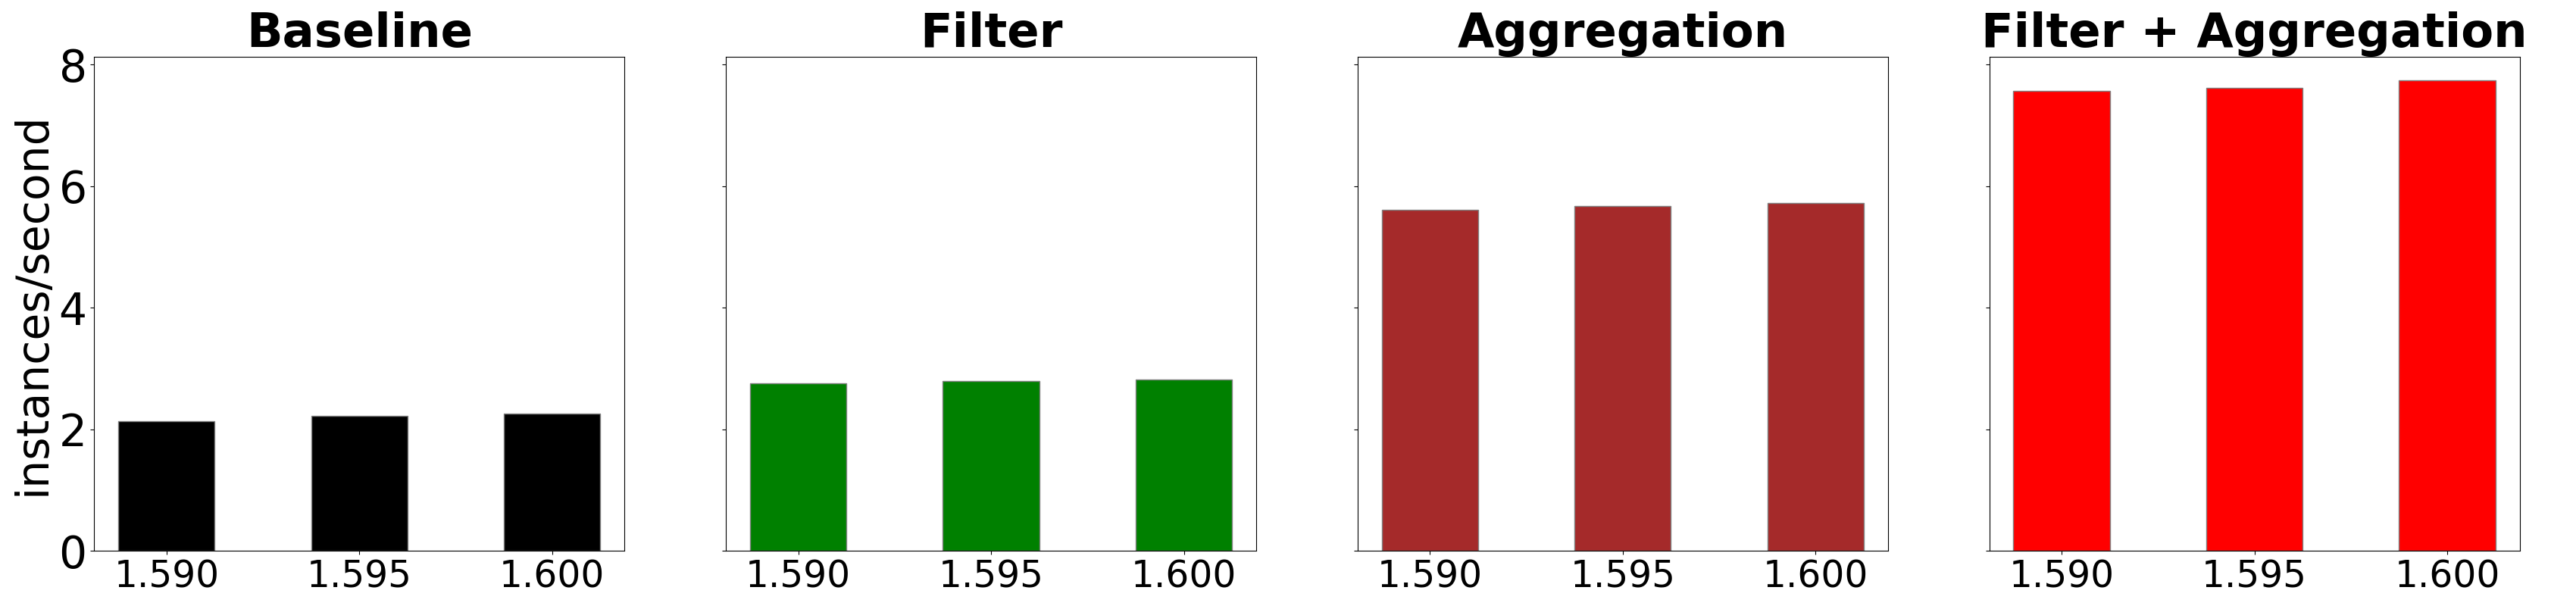
\includegraphics[height=3.5cm]{figures/topo-thr-hist-128n.png}
\vspace{5mm}

 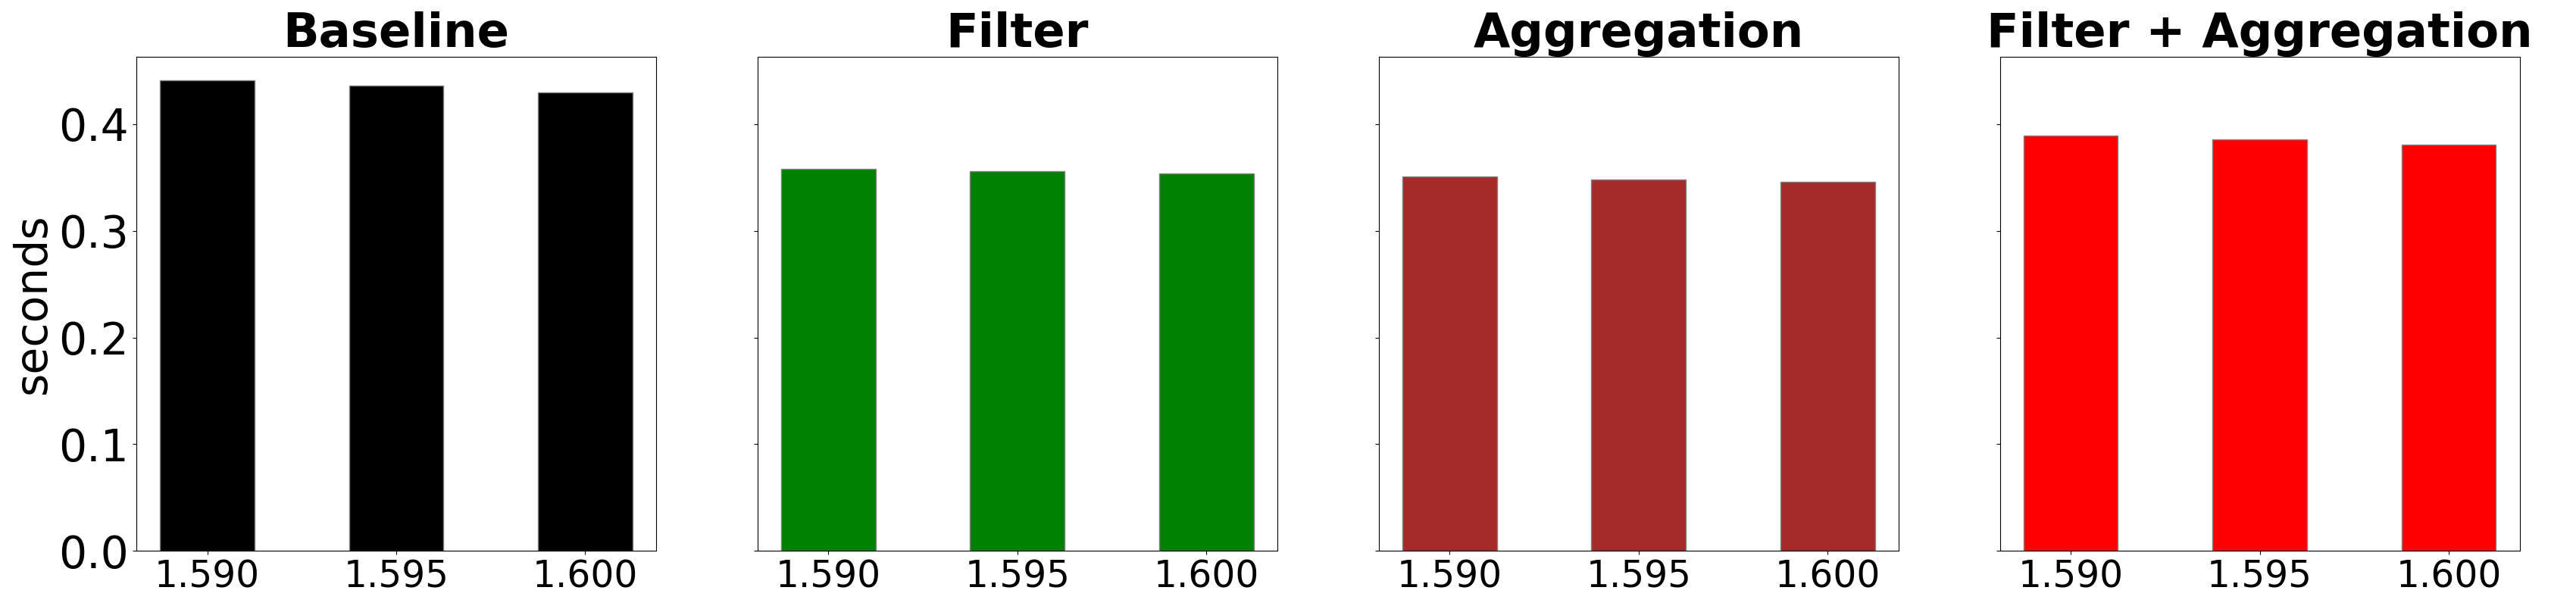
\includegraphics[height=3.5cm]{figures/topo-lat-hist-128n.png}
 
	\caption{
 Throughput (above) and latency (below) of the best throughput/latency relation points, for different setups and different average node distances (x axis for each setup) in a network with n=128 and k=51,43.}
	\label{fig:n128TopologyComparison}
\end{figure*}




% \begin{table}[h!]
% 	\begin{tabular}{c c c c c }
% 		\hline
%     Topology  &        &       &       & Filtering+  \\ 
% 	 mean & Baseline   & Filtering    & Aggregation    & Aggregation  \\  \hline

% 	1.590  		& 		...		&		&		&   \\
% 	1.595  		& 				&		&		&   \\
% 	1.600  		& 				&		&		&   \\ \hline \\
% 	\end{tabular}
% 	\caption{Saturation point throughput for different topologies, using none (Baseline), Filtering,
% 	Aggregation and Filtering and Aggregation semantic gossip mechanisms with Tendermint.}
% \end{table}


%\subsubsection{Randomness of the method -- \fd{REMOVE?}}

%Randomness is related to the overlay generation method, and not the overlay itself.  An overlay generation method is said fair if each possible edge is included in a resulting overlay with same probability. 

%An edge $(p,q)$ is included when process $p$ chooses $q$ as neighbour or vice-versa. If the assumption of proper random choice is valid, the probability of a process $p$ choosing another one $q$ as neighbour is the same for any process $q$, thus the probability that edges are included in an overlay is the same for different edges.


% The generation of the random overlay considers the set $V$ of processes, where $|V| = n$.
% The randomness is introduced by producing random permutations of the set $V$.
% This means to turning the set $V$ to an ordered set (a sequence), where the
% position of each element $v \in V$ in the ordered set is randomly chosen:

% 1. Each process $v \in V$ computes a random permutation of the set $V$ of
%    processes: `rnd_perm(v, s, V)`.
% 1. Each process $v \in V$ selects the first $k$ other processes from the
%    produced random permutation, namely `selected(v, s, k, V)` = \{ the $k$
%    first processes $p \in$ `rnd_perm(v, s, V)` with $p \neq v$ \}.

% The random network overlay is produced from the computed `selected(v, s, k, V)`
% sets, so that:

% 1. The outbound peers of process $v$ are defined by the set `selected(v, s, k, V)`.
% 1. The inbound peers of process $v$ are all processes $p \in V$ that have
%    randomly selected $v$.
%    More formally, is the set `selected_by(v, s, k, V)` =
%    \{ $p \in V$ so that $p \in$ `selected(p, s, k, V)` \}.
% 1. The set of peers of a process $v$ is: $peers_G(v)$ =
%    `selected(v, s, k, V)` $\cup$ `selected_by(v, s, k, V)`.

% Note that the same process $p$ can be on both `selected(v, s, k, V)`, thus $p$ is
% a process to which $v$ will dial, and `selected_by(v, s, k, V)`, meaning that
% $v$ should expect process $p$ to dial it.
% However, since $peers_G(v)$ is the union of the two sets, the above defined
% process $p$ should count only once as peer of $v$.
% In practical terms, this means that $v$ should keep only one of the two
% connections possibly established with process $p$.

% ## Analysis

% The source of randomness of this method is the production of the ordered sets
% `rnd_perm(v, s, V)`.
% We assume that they are actually random, so that for any two diferent processes
% $v, p \in V$, `rnd_perm(v, s, V)` and `rnd_perm(p, s, V)` are two uncorrelated
% permutations of set $V$.
% The same should apply for different random seeds `s` and `s'`, which should
% produce uncorrelated  `rnd_perm(v, s, V)` and `rnd_perm(v, s', V)`.

% If the assumption of proper random choice is valid, the probabily of $p \in$
% `selected(v, s, k, V)` should be the same for any proces $p \in V, p \neq v$.
% The probability in this case is $k/(n-1)$, as the combination of $k$ random
% selections (independent and uniform) of values from the set $V - \{v\}$, which
% contains $n-1$ elements.

% The same rationale applies for the composition of `selected_by(v, s, k, V)`.
% The probability that the process $v \in$ `selected(p, s, k, V)` is $k/(n-1)$, for
% any other process $p \in V$.
% Assuming that the production of those sets is completely independent, the
% expected number of other processes $p$ that have selected $v$ is given by the
% probability of being on each of those sets ($k/(n-1)$) times the number of
% sets considered ($n-1$).
% Thus, the expected size of set `selected_by(v, s, k, V)` is $k$, that is,
% the same size of set `selected(v, s, k, V)`.

% In term of the total number of peers, the method ensures that we have
% $|peers_G(v)| \geq k$.
% This is garanteed as |`selected(v, s, k, V)`| = k.
% To this minimal size we should add the size of set `selected_by(v, s, k, V)`,
% which expected value is $k$ as well, but removing the members from the
% intersection of both sets.
% This means that $|peers_G(v)|$ = $k$ + |`selected_by(v, s, k, V)`| -
% |`selected(v, s, k, V)` $\cap$ `selected_by(v, s, k, V)`|.

% The expectation for the number of peers $peers_G(v)$ of a process $v$ in the
% random overlay $G$ is then $2k$ minus expected size of the above mentioned
% intersection.
% To derive a more precise expectation, we would need to derive the expected size
% of the intersection `selected(v, s, k, V)` $\cap$ `selected_by(v, s, k, V)`.


\subsection{System configuration and deployment}
\label{sec:setup}

We implemented Tendermint, the gossip communication layer, and the Semantic Gossip extensions in Go.
We rely on libp2p~\cite{libp2p} to establish and maintain communication
channels between pairs of processes.
Libp2p channels are build atop TCP connections, and provide encryption,
multiplexing, flow control, and network-level batching.
Although libp2p channels are reliable, our implementation may discard messages when queues connecting different routines are full, as a way to prevent slow
processes from blocking the main transport routine.
In addition, libp2p connections may be dropped when receivers are much slower
than senders; although the dropped connections are reestablished, some messages may be lost. Temporary disconnections between peers, however, do not compromise the network connectivity.

The same Tendermint implementation is used to build different setups. In the first, \emph{Baseline}, Gossip is used. The other setups use Semantic Gossip, being \emph{Filtering} only, \emph{Aggregation} only, and 
\emph{Filtering and Aggregation} combined.
Either using Gossip or Semantic Gossip, each process opens a libp2p channel to a random subset of processes as discussed in section \ref{sec:distributedGeneration}.

The above setups are experienced with networks of 32 and a 128 nodes.
%
Load is generated at each node, upon its turn to propose a 
block for validation. I.e. whenever a node is enabled to propose a block, it does.
%
To experience higher workloads, we implemented a varying window of concurrent consensus instances allowed.
This means that while a block proposed by a node is being validated, further 
block(s) can be proposed by the next nodes.
The number of blocks that may be under validation concurrently, in the network, 
is called window.   The population of messages in intermediate nodes increases with the window sizes, allowing to better understand the effect of the mechanisms proposed.

A single instance of the experiment is characterized as a combination of: 
a given a topology (triple $\langle k, n, seed \rangle$);
one of the four setups; 
a concurrency window size; 
the time-span and the size of proposed value. 
For each combination of topology and setup, we start with window 1 and 
increment until saturation.  For each window size, 
we let the nodes free to propose and decide values as fast as possible, during a times-pan of 4 minutes.
%\fd{We use 1024 bytes as size of proposals.  ?}
%
Each node has a module where the load is generated and instances decided are 
delivered.
This allows to build an output log with all the deliveries and their consensus latencies.
%with the consensus latency for the values they generated. 
Also, during the experiment, a node periodically records working variables such as the size of the gossip queues presented with Figure \ref{fig:architecture_sg}, number of filtered messages and number of aggregated messages.


As deployment environment we use CloudLab's\cite{Duplyakin+:ATC19} bare metal machines. 
We use machines type M400 from CloudLab's Utah cluster with configuration eight 64-bit ARMv8 (Atlas/A57) cores at 2.4 GHz (APM X-GENE) and 64GB ECC Memory (8x 8 GB DDR3-1600 SO-DIMMs).


\subsection{Overall performance}
\label{sec:overall}

\begin{figure}[htbp]
	\centering
	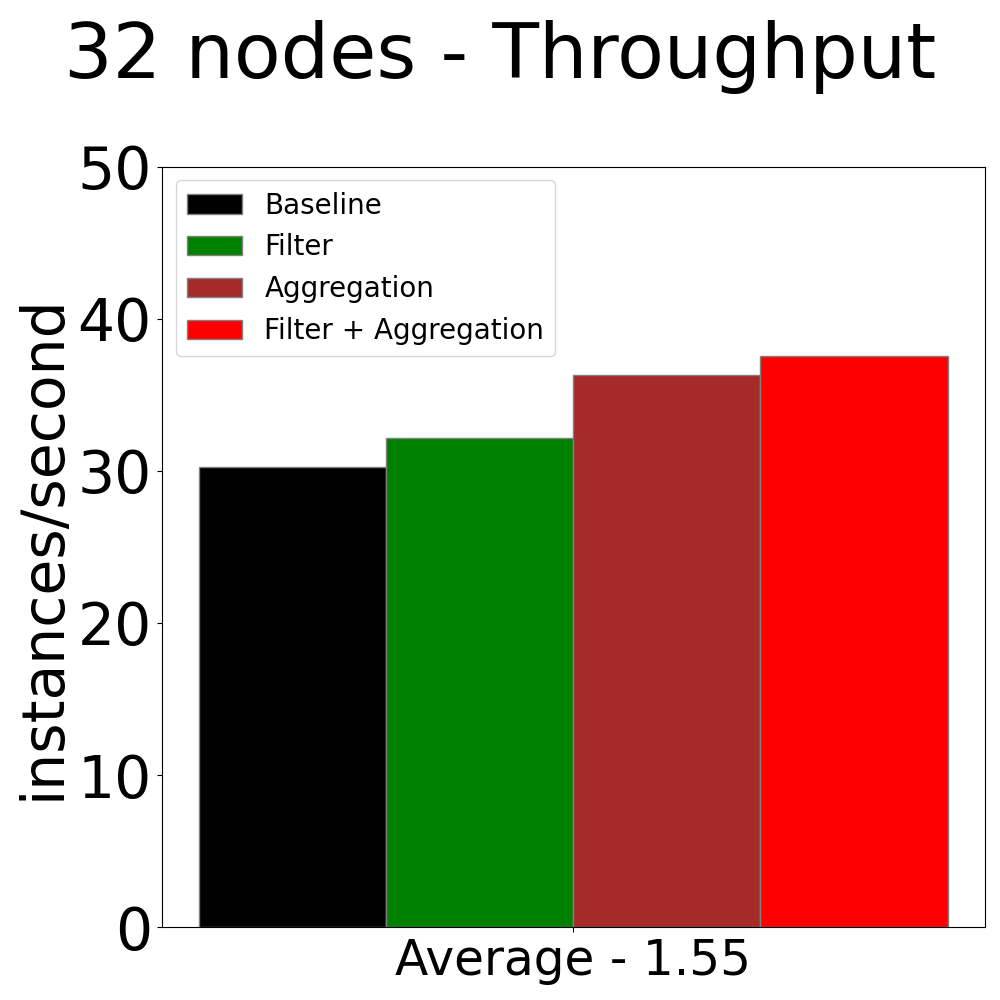
\includegraphics[%width=\columnwidth,
 height=4cm]{figures/thr-hist-32n.png}
	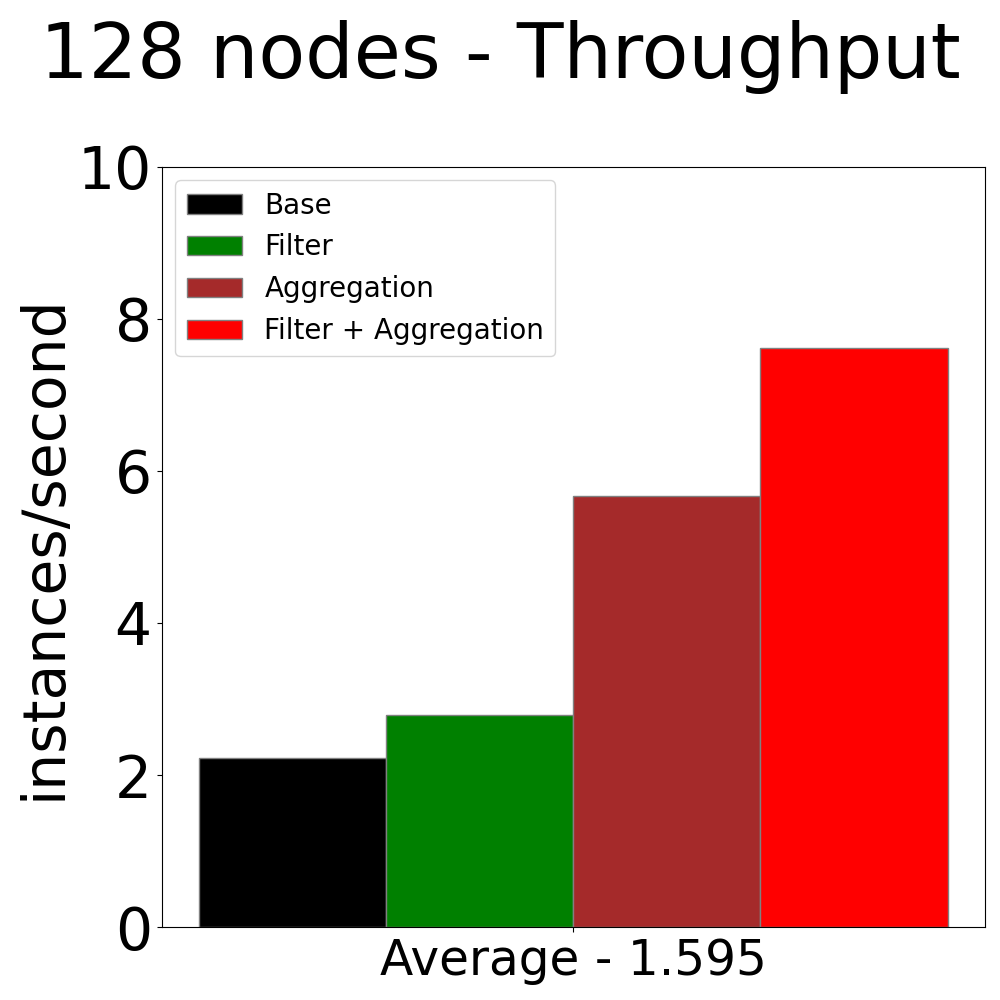
\includegraphics[%width=\columnwidth,
 height=4cm]{figures/thr-hist-128n.png}
	\caption{Comparison of throughput of the best throughput/latency relation points for Baseline, Filter, Aggregation and Filter+Aggregation for 32 (left) and 128 (right) nodes, for the average distance topology.}
	\label{fig:throughputComparisonAtSaturationPoint}
\end{figure}

Figure~\ref{fig:throughputComparisonAtSaturationPoint} shows the performance of Tendermint
in the four setups:  Baseline, Filtering, Aggregation, Filtering+Aggregation, for 32 nodes and 128 nodes.
Each bar represents the throughput at the sample with the best throughput/latency relation for each case.
This also is depicted with Table \ref{tab:sturationPoints}: for each Semantic Gossip setup,
the absolute and relative to the baseline numerical values ('relative' line) are shown.



%\begin{figure*}[htbp]
%\centering
%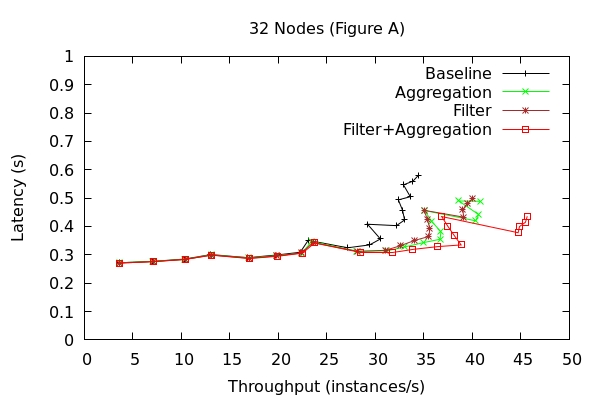
\includegraphics[width=\columnwidth]{figures/32nodes-avg-lat.png}
%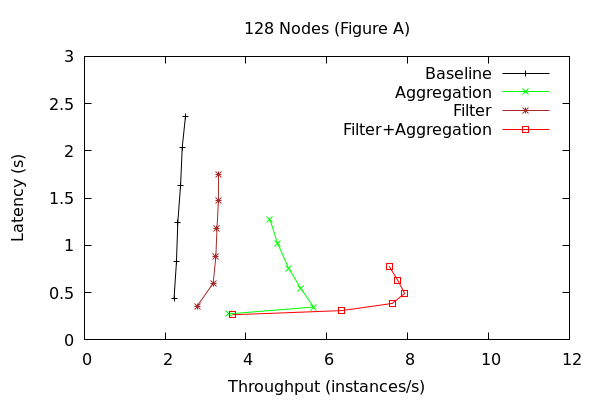
\includegraphics[width=\columnwidth]{figures/128nodes-avg-lat.png}
%\caption{Overall performance of Baseline, Filter, Aggregation and Filter+Aggregation for 32 and 128 nodes}
%\label{fig:overallTendermint}
%\end{figure*}
%
%\begin{figure*}[htbp]
%\centering
%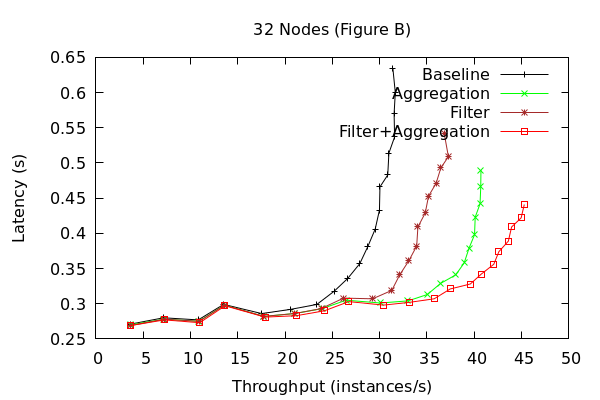
\includegraphics[width=\columnwidth]{figures/32nodes-eq-lats.png}
%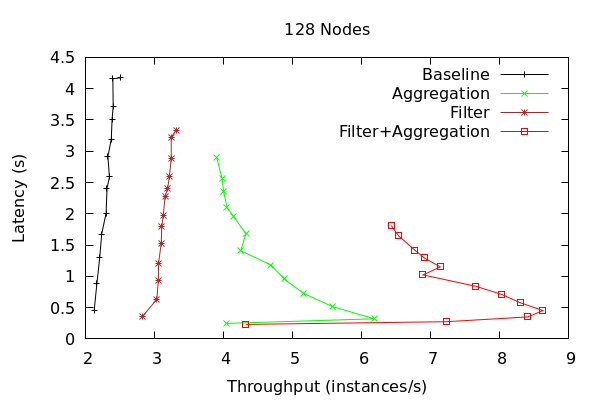
\includegraphics[width=\columnwidth]{figures/128nodes-eq-lats.png}
%\caption{Overall performance of Baseline, Filter, Aggregation and Filter+Aggregation for 32 and 128 nodes when all regions have equal latency between them}
%\label{fig:overallTendermintEqLats}
%\end{figure*}
%\rg{For 32 nodes it seems that using different latencies between regions have caused the issue of throughput decreasing and increasing "randomly", and the second plot shows something closer to our expectations. In the 128 nodes case the behaviour was essentially the same, but I ran the experiment with more points(more window sizes, up to 13). What I think is happening is that the aggregation is becoming less and less efficient as we increase the number of messages traveling on the network, because as we have more instances running concurrently we reduce the probability of a message be "close" in a receive buffer to other "aggregatable" messages. }
%
%\fd{For 32 nodes we experimented window varying from 1 to 20.  As can be seen, the throughput latency behavior has atypical variations.  In Fig 6, left, we show results for the same experiment, but adopting homogeneous latencies for all links in the topology.  As the window increases, different leaders are involved in ongoing instances. If a certain window size concentrates high latency leaders, its corresponding performance could be penalized.
%
% }

% \begin{figure}[htbp]
% \centering
% 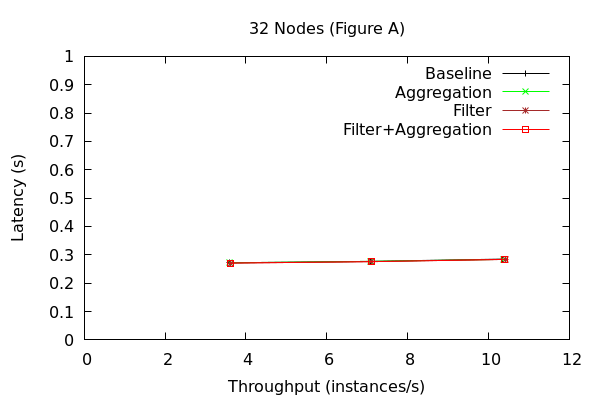
\includegraphics[width=\columnwidth]{figures/32nodes-3points.png}
% \caption{Close up of system performance with 32 nodes in the first three window sizes}
% \label{fig:cdfsW11}
% \end{figure}

%In the experiments with 32 nodes,
%the four setups perform almost equally until the Baseline reaches saturation (window  $\approx 10$, $\approx 30$ instances per second). 
With 32 nodes, the Baseline saturation point is reached with window 10, with several nodes showing average load\footnote{Linux measure meaning the number of processes which are either currently being executed by the CPU or are waiting for execution.} above the number of cores (8 in our experiment) revealing contention for CPU.  We also observed that  message handling is a main factor to CPU utilization.
%
As the mechanisms proposed spare messages, the demand for CPU is alleviated.   Thus, setups Filtering and Aggregation, in isolation, allow to further scale.  The combination of both, Filtering+Aggregation, leads to better performance than the isolated cases, reaching throughput 
1.24 $\times$ faster than the Baseline while slightly reducing latency.     

In experiments with 128 nodes the same is observed.  Due to the high number of nodes and consequent message handling demand, the Baseline setup shows saturation starting from window 1, again with average CPU load above the number of cores for several nodes.  Filtering and Aggregation alone again show positive results, shrinking latency and enhancing throughput.   Their combination allowed to reach 3.42 $\times$ the Baseline throughput showing latency compatible with 32 nodes on non-saturated setups.

\begin{table}[h!]
\centering
	\begin{tabular}{c c c c c }
	\hline
     Size in     &        &       &       & Filtering+  \\ 
	 Nodes & Baseline   & Filtering    & Aggregation    & Aggregation  \\  \hline
	32  		& 		30.261		&	32.145	&	36.271	&  37.559 \\
	relative   		& 		  1		&	1.06	&	1.20	&  1.24      \\ \hline
	128  		& 		2.223		&	2.791	&	5.672	&  7.618  \\  
	relative   		& 		  1		&	1.25	&	2.55	&  3.42  \\ \hline \\
 
	\end{tabular}
	\caption{Tendermint throughput for different network sizes and  gossip setups, at the best throughput/latency point.}
 \label{tab:sturationPoints}
 \vspace{-5mm}
\end{table}

\subsection{Mechanisms Working}

To better understand the effect of the mechanisms, we take the points with best throughput/latency relation and quantify their impact on message handling.   

Regarding Filtering, the results for setups Filtering and Filtering+Aggregation are depicted in Table \ref{tab:Filtering}.
With the 32 nodes network it shows that around 23\% of the messages were filtered out in both setups, while with 128 nodes around 30\% of the messages were filtered out.

\begin{table}[h!]
\centering
	\begin{tabular}{c c c c c }
	\hline
     Size in     &       &  Filtering+  \\ 
	 Nodes & Filtering    & Aggregation  \\  \hline
	32  		&	23.07\%	&  23.17\% \\
	128  		&	29.87\%	&  28.81\%  \\ \hline \\
	\end{tabular}
	\caption{Percentage of messages filtered out by the semantic filter mechanism at the best throughput/latency point.}
  \label{tab:Filtering}
\vspace{-3mm}
\end{table}

With Aggregation, we can observe in Table \ref{tab:Aggregation}
that the share of messages aggregated with others 
importantly increases with the number of nodes, revealing that indeed the phased and symmetric structure of the protocol lends itself for the usage of the Aggregation technique.

\begin{table}[h!]
\centering
	\begin{tabular}{c c c c c }
	\hline
     Size in     &       &  Filtering+  \\ 
	 Nodes & Aggregation    & Aggregation  \\  \hline
	32  		&	16.77\%	&  13.01\% \\
	128  		&	70.92\%	&  71.76\%  \\ \hline \\
	\end{tabular}
	\caption{Percentage of messages aggregated  at the best throughput/latency point.}
   \label{tab:Aggregation}
 \vspace{-5mm}
\end{table}
%\fd{just reminding.  this is the percentage of messages that were aggregated with others.  it does not measure exactly how many less messages were sent due aggregation.}

% \rg{One thing that maybe is interesting to mention here is that we have 23\% on the execution that were filtered out and we also have a difference of 24\% between the recvMsg/(numNodes*instances) ratios of the Baseline and the Filtering(19.25/25.14 at table III). In other words, as we skip sending 23\% of the messages, the nodes receive 24\% less messages per instance in comparison to the Baseline. Same way, we had 30\% of messages filtered out for 128 nodes and they received 33\% less messages per instance compared to the Baseline.}

% \fd{yes ... i am thinking that table II seems a fundamental measure  and maybe other measures just collapse to that...}


\subsection{Gossip messages per consensus instance}

To further evaluate the impact, we compute the average number of gossip messages received per node to complete a consensus instance. 

In an analytical approximation, for a network of $n$ nodes, each of which having $k$ neighbors, 
considering that a gossiped message reaches every node and each node forwards it once to its neighbors, we have that in average every node should receive $n * k/n = k$ copies of a gossiped message.
%
%Now, considering that we have one gossip diffusion for the $Propose$ step and $n$ gossips for the $Prevote$ and $Precommit$ steps, our estimation is that for every instance of consensus a node should receive $2nk$ gossiped messages. 
Now, considering that after the $Propose$ by the coordinator, each of the $n$ nodes gossips the $Prevote$ and then gossips the $Precommit$, our estimation is that for every instance of consensus a node should receive $2nk$ gossiped messages. 
For instance, with $n =32$ and $k = 13.87$, a consensus instance would lead each node to receive 
$\sim 887$ messages, while with $n =128$ and $k = 51.43$, would be $\sim 13.166$ messages.
However, as a node doesn't need every message to progress, and, depending on messages received, may skip phases, this upper bound should not be meet in practice.

In Table \ref{tab:msgsRcvdPerInstance} we depict the observed number of gossip messages handled per node, per consensus instance, for the several setups.   The baseline values are 7,9\% and 2,8\% under the estimated upper bound.
We notice that Filtering showed reduction  of 26\% and 31\% of messages respectively for 32 and 128 nodes. As discussed, 
Aggregation shows high impact as the number of nodes increase, here with 17\% and 75\% less messages for 32 and 128 nodes respectively.  Again, the mechanisms combined show still better effect than in isolation for both network sizes.

%\rg{Note that a network is built from a number $n$ of nodes, each of which has $k$ neighbors, each message is sent only once and every process should receive this message eventually. Thus every node should receive $n * k/n = k$ messages every time another node gossips a message. The number of gossip attempts per instance is $2n$, since we have one gossip diffusion for the $Propose$ step and $n$ gossips for the $Prevote$ and $Precommit$ steps. So our estimation says that for every instance of consensus a node should receive $2nk$ gossiped messages. But we should never meet this upper bound is practice, because a node doesn't needs every message to progress, only two thirds.}

%\rg{It seems that the filtering is more effective in smaller networks and aggregation in bigger ones. Another thing worth mentioning is that the aggregation is less and less effective as we increase the concurrency window size, as it is "opportunistic" in it's way of selecting the messages it should aggregate(it looks for the first 500 or something inside the "sendMessageBuffer"). }
%\fd{too much detail for this version}

\begin{table}[h!]
\center
	\begin{tabular}{c c c c c c }
	\hline
     Size in   & Estimated &   Base-    & Filte-      & Aggre-     & Filter.+  \\ 
	 Nodes & upper bound &     line   &   ring     &   gation    & Aggreg.  \\  \hline
	32  		& 887 & 		822,2        &	612,6	&	690,6	&  537,9 \\
 	relative   	& 1,079    & 		  1		     &	0,74	&	0,83	&  0,65      \\ \hline
	128  		& 13.166 & 		12.805,4   &	8.876,3	&	3.613,1	&  2471  \\ 
 	relative   	&  1,028   & 		  1		     &	0,69	&	0,25	&  0,19      \\ \hline \\
	\end{tabular}
	\caption{Average of gossip received messages per node, per decided Tendermint instance, at the best throughput/latency point.}
  \label{tab:msgsRcvdPerInstance}
 \vspace{-5mm}
\end{table}


\subsection{Latencies}
\label{sec:latency-cdfs}

Window 1 represents the situation where an instance of consensus is proposed only after the previous has been finished, therefore with minimum contention.
%
For 32 nodes and window 1, we observe in Figure \ref{fig:cdfs}(center) that all setups have the same latency distribution (lines are collapsed).  This means that the semantic mechanisms neither help nor impacted latency in this light scenario.

Interestingly, from Figure \ref{fig:cdfs} we observe that with 128 nodes, window 1 (right), the setups with Aggregation show latency distribution very similar to the reported with 32 nodes, window 1 (center), while the Filtering and Baseline show higher latency, in this order.
%
This emphasizes the 
importance of Aggregation as the number of nodes grows.  As Tendermint uses communication steps with the same types of messages addressed to all participants, the population of messages prone to Aggregation in intermediate nodes, and thus the positive impact of Aggregation, is proportional to the number of nodes.  
%

%leaving to conclude that Aggregation 
%this setup reduced communication overhead to be compatible with having $1/4$ of nodes.

%\fd{really?}   \rg{I think that saying it's "compatible with another size" it's a little bit problematic because the number of messages depends on K as well, and also the number of gossiped messages per instance of 128 nodes with filter+aggreg is three times the theoretical upper bound(2kn) we have for 32 nodes when k is 9. So, saying its "compatible with N" without specifying a K it's not very precise. What I think we can say is that we ...?  }

To detail the behavior with 32 nodes we take from the less performing setup (Baseline) the window with best throughput/latency point (window 13).
With this configuration all setups show similar throughput.
The latency distributions of the four setups is depicted in Figure \ref{fig:cdfs} (left).  %As the Baseline reaches saturation, 
Latency distributions are slightly better using Semantic Gossip. Aggregation shows  better impact than Filtering, and their combination further reduces latency.   

An important general observation is that the mechanisms are not delaying instance's decision, even if messages are dropped due to filtering.  On the contrary, latency distributions are consistently better at all percentiles with the mechanisms proposed, showing that sparing redundancy is indeed possible and a good measure.

\begin{figure*}[htbp]
\centering
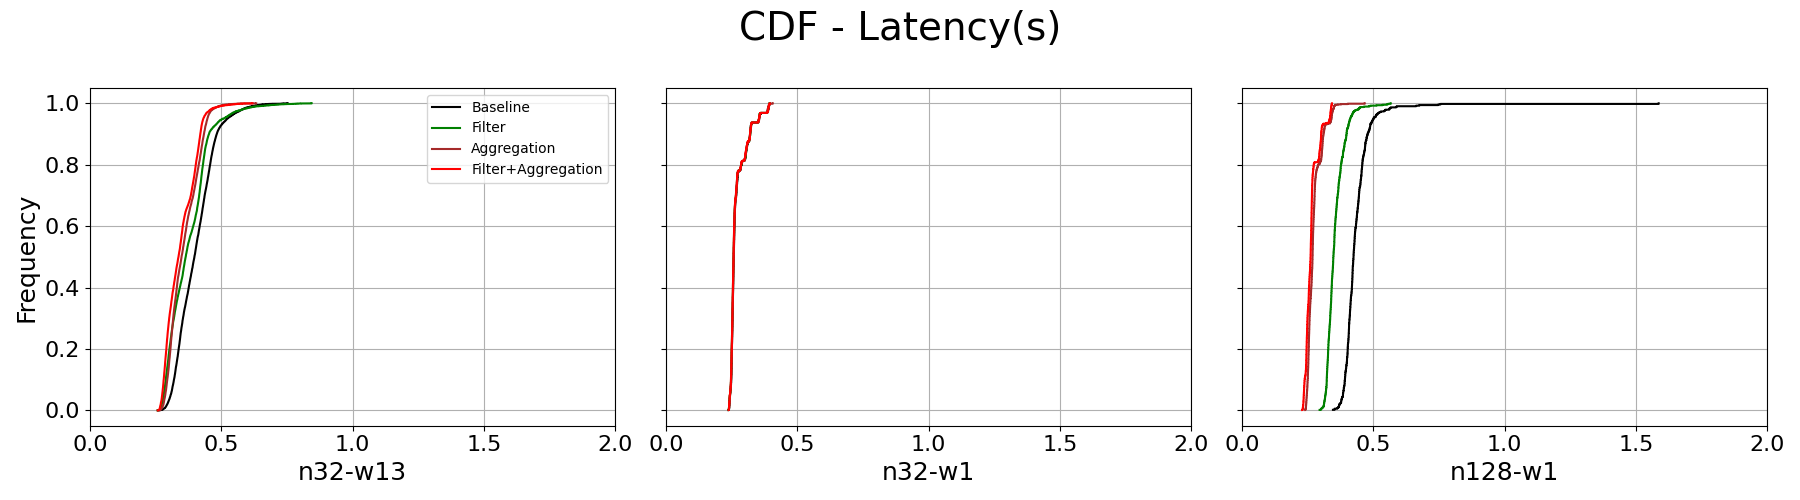
\includegraphics[width=\textwidth, height=4cm]{figures/cdfs.png}
\caption{Latency CDFs for Baseline, Filter, Aggregation and Filter+Aggregation, using window 13 for 32 nodes (left), window 1 for 32(center) and window 1 for 128 nodes(right)}
\label{fig:cdfs}
\end{figure*}


% \begin{figure*}[htbp]
% \centering
% 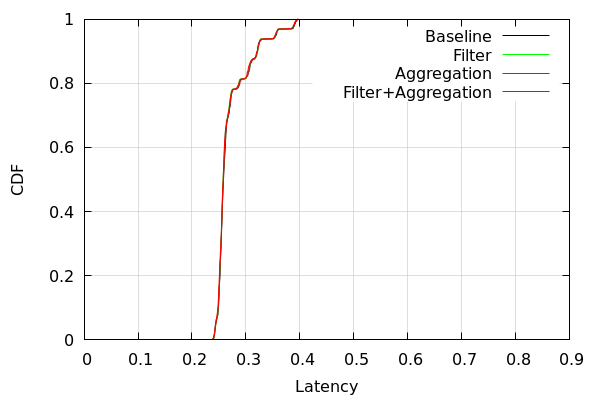
\includegraphics[width=\columnwidth]{figures/w1-32nodes-cdf.png}
% 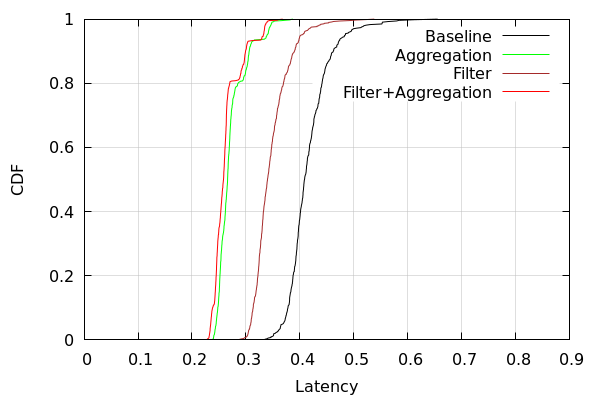
\includegraphics[width=\columnwidth]{figures/128nodes-cdf.png}
% 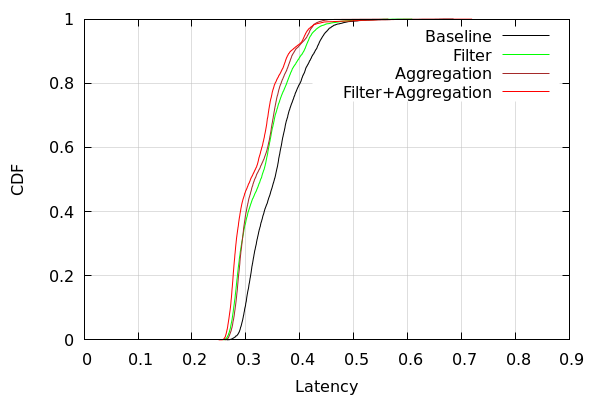
\includegraphics[width=\columnwidth]{figures/w11-32nodes-cdf.png}
% \caption{Latency CDFs for Baseline, Filter, Aggregation and Filter+Aggregation, using window 1 for 32 nodes (left) and  128 nodes(right)}
% \label{fig:cdfs}
% \end{figure*}

% \begin{figure}[htbp]
% \centering
% \caption{Latency CDf for 32 nodes Window size 11}
% \label{fig:cdfsW11}
% \end{figure}

\subsection{Resilience}
\label{sec:resilience}
\fd{SHOULD WE KEEP THIS OR DO THE MESSAGE LOSS STUDY?}

As redundancy is needed to cope with byzantine behavior and since Semantic Gossip is designed to safely eliminate redundancy, we designed experiments to evaluate if and how consensus is affected by byzantine behavior using Semantic Gossip mechanisms in comparison to the Baseline.

Under the assumption that signatures are reliable and since gossip works with signature verification, any attempt to forge or corrupt messages would be detected.   Therefore, we conclude the worst byzantine behavior to harm consensus would be that dishonest nodes remain silent, i.e. they do not collaborate with the consensus protocol.

For 32 and 128 nodes, we incrementally convert honest to byzantine nodes, 5 by 5\%, starting with 0 and going up to 30\%.  Regardless of performance, consensus should show progress in all cases since it supports up to $1/3$ dishonest nodes.  Tables \ref{tab:biz32} and \ref{tab:biz128} show the resulting throughput of the experiment respectively for 32 and 128 nodes.  The first general observation is that all configurations keep progress.   The second is that for 128 nodes all Semantic Gossip configurations performed better than or equivalent to the Baseline.  Thirdly, for 32 nodes, in all configurations the effect of having Filtering+Aggregation slightly enhanced or has equivalent throughput.   For Filtering and Aggregation separated, in most cases performance was equivalent or better than the Baseline.  For 30\% dishonest nodes these setups show performance below the Baseline, indicating that message drop by the mechanisms, added by 30\% of silent nodes, have slightly delayed consensus to be reached.

\begin{table}[h!]
\centering
	\begin{tabular}{c c c c c }
	\hline
     Byzantine     &        &       &       & Filtering+  \\ 
	 Nodes & Baseline   & Filtering    & Aggregation    & Aggregation  \\  \hline
	 0 \%  		    & 		1		&	1	&	1	& 1  \\
	 5 \%  		    & 		0.044		&	0.041	&	0.040	& 0.037  \\
	 10 \%  		& 		0.022		&	0.020	&	0.021	& 0.019  \\
	 15 \%  		& 		0.022		&	0.020	&	0.020	& 0.018  \\
	 20 \%  		& 		0.021		&	0.017	&	0.019	& 0.018  \\
	 25 \%  		& 		0.017		&	0.019	&	0.023	& 0.023  \\
	 30 \%  		& 		0.017		&	0.010	&	0.009	& 0.016  \\ \hline \\
	\end{tabular}
	\caption{Tendermint throughput in instances/sec with 32 nodes. 
 Each setup with window of best throughput/latency point with 0 dishonest nodes.   Then converting nodes 5 by 5\% to dishonest.}
 \label{tab:biz32}
\end{table}

\begin{table}[h!]
\centering
	\begin{tabular}{c c c c c }
	\hline
     Byzantine     &        &       &       & Filtering+  \\ 
	 Nodes & Baseline   & Filtering    & Aggregation    & Aggregation  \\  \hline
	 0 \%  		    & 		1		&	1	&	1	& 1  \\
	 5 \%  		    & 		0.329		&	0.249	&	0.173	& 0.131  \\
	 10 \%  		& 		0.200		&	0.153	&	0.094	& 0.065  \\
	 15 \%  		& 		0.157		&	0.115	&	0.075	& 0.051  \\
	 20 \%  		& 		0.116		&	0.085	&	0.051	& 0.035  \\
	 25 \%  		& 		0.100		&	0.073	&	0.042	& 0.039  \\
	 30 \%  		& 		0.083		&	0.068	&	0.062	& 0.052  \\ \hline \\
	\end{tabular}
	\caption{Tendermint throughput in instances/sec with 128 nodes. 
 Each setup with window of best throughput/latency point with 0 dishonest nodes.   Then converting nodes 5 by 5\% to dishonest.}
  \label{tab:biz128}
\end{table}



% \fd{a análise acima é válida.   acho que podemos seguir pela vazao.
% adicionando grafico de thoughput/latencia podemos mostrar que os mecanismos nao prejudicam latencia}


% talvez possamos usar latencia ...

% PARA RESPONDER QUE OS MECANISMOS NAO IMPEDEM A DECISAO,  PODEMOS PEGAR O CASO DE JANELA 1 E VER A LATENCIA PARA DECISOES.   SE A LATENCIA PARA DECISAO FOR MAIOR QUE PARA O BASELINE, EM TESE ALGUMA MENSAGEM ESTA SENDO JOGADA FORA E NAO DEVERIA.   SE TIVER LATENCIA MELHOR, AINDA MELHOR.

% UM ESTUDO ADICIONAL SERIA SUPONDO O SISTEMA EM ALTA UTILIZCAO, COMO IMPACTAM OS BIZANTINOS EM CADA CASO.
% AQUI PEGARIA O CENARIO DE MELHOR THROUGHPUT/LATENCIA EM CADA CASO.
% DAI TERIA QUE PLOTAR O GRAFICO THROUGHPUT/LATENCIA,
% E UMA TABELA DE LATENCIA MEDIA POR INSTANCIA. 


\subsection{Message loss}
\label{sec:msgLoss}
In addition to Byzantine behaviors, a consistent consensus mechanism must also be tolerant of imperfect links that allow message loss. We implemented this feature by dropping messages, when they are received, with a predefined probability, so they are not computed by the consensus neither forwarded to other peers.   We measure latency and throughput of the different techniques with loss probabilities increasing 5 by 5 from 0 to 60\%, in a network of 32 nodes.   With window 1,   we observe a gradual degradation of the performance, both for throughput and latency, until we arrive at 50 to 60\% message loss.   With window 13,  
%
%This way, we are able to measure the impacts of faulty links on Tendermint's performance, with and without the Semantic Gossip techniques. 
%
%Now, since the Semantic Filtering reduces the total amount of messages per consensus instances to the minimum needed for termination and Semantic Aggregation may lead to several messages being dropped at once, we also evaluate whether these techniques make the system more susceptible to postponement due to message loss.
%
%We incremented the message loss probability 5 by 5\%, starting from 0, but going up to 60\%. We evaluated this scenario exclusively for the 32 nodes configuration because...(should we argue something here?). 
Figures \ref{fig:msgLossThroughput} and \ref{fig:msgLossLatency} show that we have a gradual degradation of the performance,  until we arrive at 30\% message loss, where the number of decided instances drops abruptly. The baseline has this threshold point with 35\% message loss. 
%
%This behavior is spread among all the experimented setups, which leads us to the conclusion that no vulnerability was introduced by our Semantic Gossip module regarding message loss tolerance. 
%
This shows that, with Semantic Gossip filtering and aggregation, the system operates with performance better than the Baseline even under loss rates up to 30\%.


%the degree of redundancy of the gossip propagation method is very high, allowing the system to operate with performance similar to the case without failures with up to 30\% message loss.\fd{revise this ...}


%\begin{figure}[htbp]
%	\centering
%	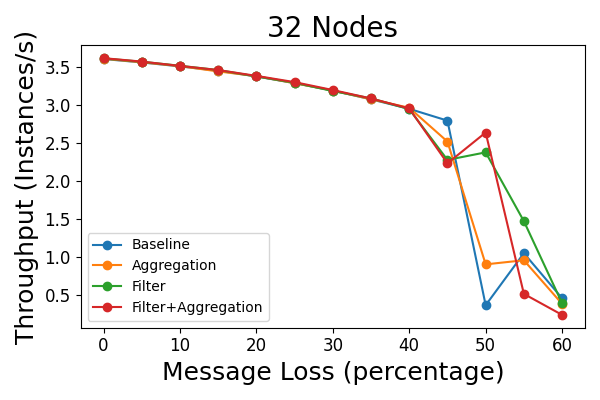
\includegraphics[%width=\columnwidth,  height=5cm]{figures/msgloss-diff-lat-32nodes-loss-thr.png}
	
%\caption{Tendermint throughput in instances/s with 32 nodes. Setups with window size equals one. Message loss percentage incremented 5 by 5.}
	%\label{fig:msgLossThroughput}
%\end{figure}

%\begin{figure}[htbp]
%	\centering  
	%\includegraphics[%width=\columnwidth, height=5cm]{figures/msgloss-diff-lat-532nodes-loss-lat.png}
%	\caption{Tendermint latency in seconds with 32 nodes. Setups with window size equals one. Message loss percentage incremented 5 by 5.}
	%\label{fig:msgLossLatency}
%\end{figure}



\begin{figure}[htbp]
	\centering
	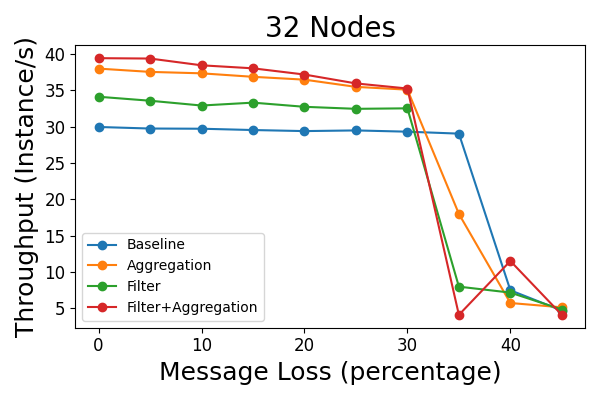
\includegraphics[%width=\columnwidth,
  height=5cm]{figures/w13-msgloss-32nodes-loss-thr.png}
	\caption{Tendermint throughput in instances/s with 32 nodes. Setups with window size equals 13. Message loss percentage incremented 5 by 5.}
	\label{fig:msgLossThroughput}
\end{figure}

\begin{figure}[htbp]
	\centering  
	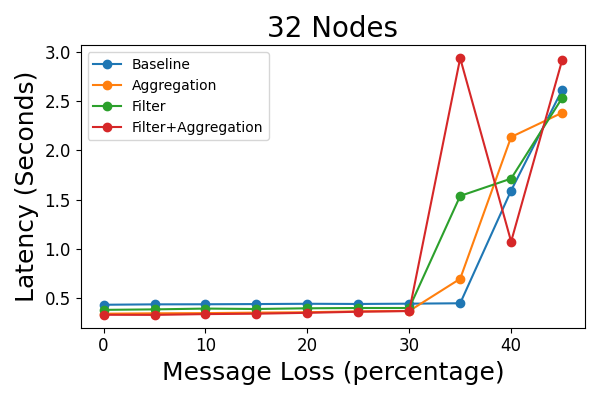
\includegraphics[%width=\columnwidth, 
     height=5cm]{figures/w13-msgloss-32nodes-loss-lat.png}
	\caption{Tendermint latency in seconds with 32 nodes. Setups with window size equals 13. Message loss percentage incremented 5 by 5.}
	\label{fig:msgLossLatency}
\end{figure}

\label{sec:signatureImpact}


% \begin{table}[h!]
% 	\begin{tabular}{c c c c c }
% 	\hline
%      Signature     &        &       &       & Filtering+  \\ 
% 	 Validation & Baseline   & Filtering    & Aggregation    & Aggregation  \\  \hline
% 	  on  		& 		...		&		&		&   \\
% 	  off  		& 				&		&		&    \\ \hline \\
% 	\end{tabular}
% 	\caption{Saturation point throughput using signature validation, or not, with 
% 	none (Baseline), Filtering,
% 	Aggregation and Filtering and Aggregation semantic gossip mechanisms with Tendermint.}
% \end{table}

% \rg{We have to discuss better the data. }




%!TEX root =  report.tex
\section{Related work}
\label{sec:relwork}
\color{teal}
Gossip algorithms were first introduced by Demers et al.~\cite{demers87} to
manage replica consistency in the Xerox Clearinghouse Service~\cite{oppen83}.
The proposed algorithms were specific for the dissemination of database
updates, assumed to not be very frequent (a few per second, at most).
%
The adoption of gossip mechanisms as a building block for the dissemination of
arbitrary application messages derives from Bimodal Multicast~\cite{Birman99}.
The algorithm consists of two phases.
In the first phase, messages are disseminated in a best-effort fashion through
multicast trees, using IP-multicast when available.
In the second phase, processes periodically send to a random-selected peer a list
of recently received messages, so that to retransmit, on demand, messages that
have not yet been received by the peer.
%
Since then, multiple approaches have been proposed to improve throughput and
robustness of gossip dissemination~\cite{birman01, eugster03, gupta02, kempe04,
lin99, leitao07, melamed04, vogels03}.

Research in gossip-based broadcast algorithms has focused essentially on two
issues.
%
First, the efficient dissemination of messages in large-scale systems through
the adoption of overlay networks.
Proposed approaches consider building pseudo-random network overlays,
by selecting links based on geographic proximity and available
bandwidth~\cite{kempe04, melamed04}, or topological and connectivity
properties~\cite{lin99, leitao07, voulgaris13}.
%
A second research direction addresses the cost/effectiveness of epidemic
mechanisms which enable processes to request messages that they failed to
receive.
The efficiency of these anti-entropy~\cite{demers87, Birman99} or gossip
repair~\cite{birman01, eugster03, gupta02, vogels03} mechanisms
is crucial to improve the reliability of gossip dissemination.
%
Efforts have also been made to develop gossip-based services to support
large-scale broadcast and multicast algorithms, such as failure
detection~\cite{renesse98}, group membership~\cite{ganesh03, johansen06},
monitoring and management systems~\cite{renesse02}.

Semantic Gossip differs from existing approaches because it is designed to
support distributed applications that, by themselves, include layers of
redundancy.

\color{black}

This is the case of Paxos, which includes both typical broadcast steps (to
propose values) and the exchange of control messages to ensure agreement, which
is a strong form of reliability.

Probabilistic Atomic Broadcast~\cite{felber02} is the algorithm whose behavior
most resembles the operation of Paxos atop gossip.
%is most similar to 
The algorithm proceeds in rounds, in each round a process can broadcast a
message and should vote for a message, either broadcast or received during the
round.
Processes periodically exchange the list of messages and associated votes with
a random subset of peers.
When the number of votes reaches a threshold, all messages in the list are
delivered, and the process proceeds to the next round.
%
As in our Paxos deployment, processes send and forward values (broadcast
messages) and votes to peers via gossip.
Unlike Paxos, the algorithm of~\cite{felber02} only provides probabilistic
safety guarantees: two processes may deliver messages in distinct orders, which
is equivalent in Paxos to deciding different values in the same consensus
instance.

\color{teal}

Even though most work on gossip has considered benign failures (e.g., process crashes), 
recent Byzantine fault tolerant consensus protocols for large-scale environments (e.g., blockchain) 
have considered the use of gossip as underlying communication substrate.
Tendermint
%\footnote{\url{https://tendermint.com/}} 
is a blockchain middleware
based on a BFT consensus algorithm~\cite{bucham18} designed for gossip
communication.  Tendermint has its own gossip layer implementation, that is
application-specific and tightly coupled with the consensus implementation.
%
Casper~\cite{buterin17}, the BFT consensus algorithm proposed to replace the
proof-of-work core of the Ethereum blockchain is also designed for a
gossip-based environment.
%\footnote{\url{https://ethereum.org/}}
%
HotStuff~\cite{maofan18}, the BFT consensus protocol at the core of the Libra
Blockchain~\cite{amsden20}, although not designed for gossip-based
communication, considers its adoption as the number of processes participating
on consensus (validator nodes) grows~\cite{libra18}.
The key architectural aspect that distinguishes these proposals from Semantic
Gossip is that gossip in blockchain systems is intertwined with consensus
logic.  Semantic Gossip exploits application (i.e., consensus) semantics
without giving up modularity.

\color{black}

%!TEX root =  report.tex
\section{Conclusions}
\label{sec:conclusions}
\color{teal}
This paper introduces Semantic Gossip, a communication substrate that takes application semantics into account to optimize performance.
Semantic Gossip relies on two techniques, semantic filtering and semantic aggregation.
With semantic filtering, the gossip protocol can stop propagating messages that have become redundant from the perspective of the application.
With semantic aggregation, the gossip protocol can replace multiple messages by a single message of equivalent meaning.
Both techniques reduce the number of messages that are propagated by gossip without penalizing the resilience of the consensus protocol.
\color{black}

We have demonstrated the usefulness of Semantic Gossip using Tendermint, a well-known consensus protocol.  It enables to scale ...




%\section*{Acknowledgments}
%This work was partially supported by the Swiss National Science Foundation (\# 175717), Funda\c{c}\~{a}o de Amparo \`{a} Pesquisa do Estado Do Rio Grande do Sul---FAPERGS PqG 07/21, Conselho Nacional de Desenvolvimento Cient\'{i}fico e Tecnol\'{o}gico---CNPq Universal 18/21, PUCRS-PrInt,  Coordena\c{c}\~{a}o de Aperfei\c{c}oamento de Pessoal de N\'{i}vel Superior (CAPES), Brazil, Finance Code 001, and FAPDF through EDITAL 08/2023---FAP Participa.

%% the bibliography file.
\bibliographystyle{wileyNJD-AMA}
\bibliography{report}

\section{Author Biography}

\begin{biography}{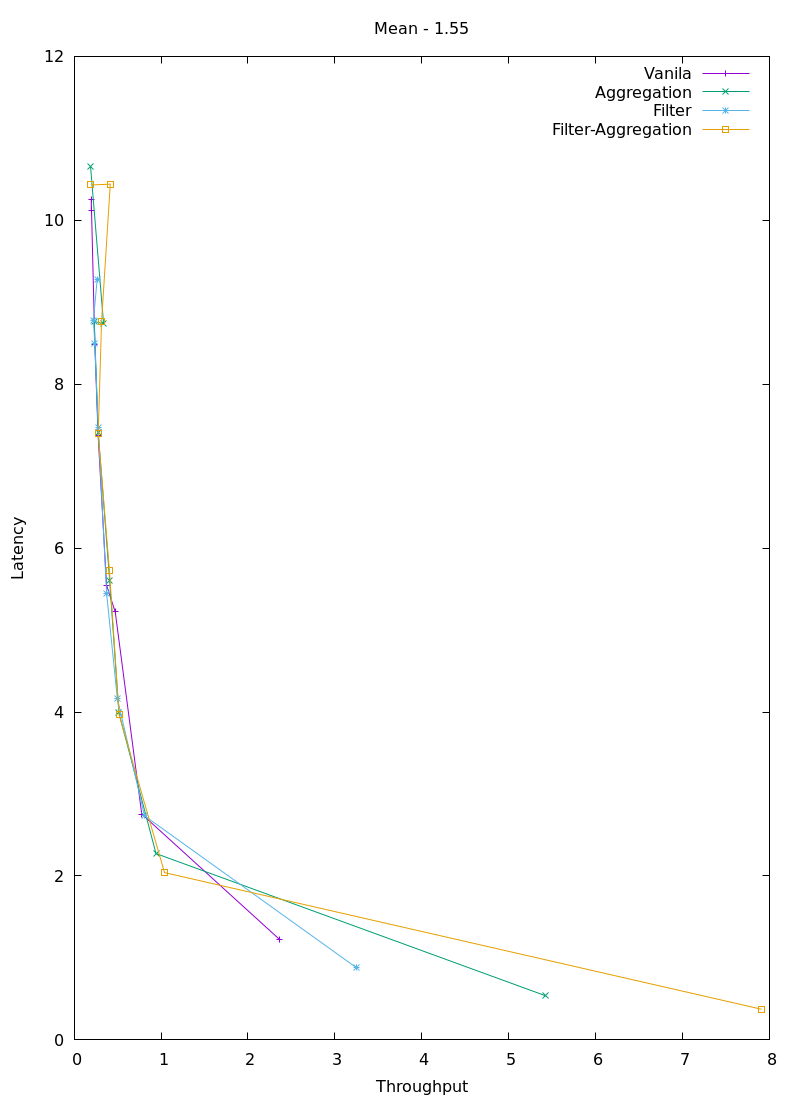
\includegraphics[width=76pt,height=76pt,draft]{figures/128nodes-byzantine.png}}
      {\textbf{Author Name.} Please check with the journal’s author guidelines
      whether author biographies are required. They are usually only
      included for review-type articles, and typically require photos
      and brief biographies for each author.}
\end{biography}


\end{document}


